\section{Verification of model}
\label{verification_of_model}

A model of the water distribution system is obtained, this has now been linearized, \secref{Linearization}, the parameters have been estimated, \secref{LinParamEst}, the model is arranged on SS form, \secref{SystemLin_control}, and finally discretized, \secref{discrete_SS}. In this section the model is excited in different ways, to consider if the behavior is deemed reasonable compared to the test setup. First the time constant for the WT is compared to real measurements, then an input is applied to both pumps in order to see how the pressure at the CP changes and then the disturbance, given as OD of the values, is changed to see how the pressure at the CP changes. 

\begin{figure}[H]
   \centering
    % This file was created by matlab2tikz.
%
%The latest updates can be retrieved from
%  http://www.mathworks.com/matlabcentral/fileexchange/22022-matlab2tikz-matlab2tikz
%where you can also make suggestions and rate matlab2tikz.
%
\definecolor{mycolor1}{rgb}{0.00000,0.44700,0.74100}%
%
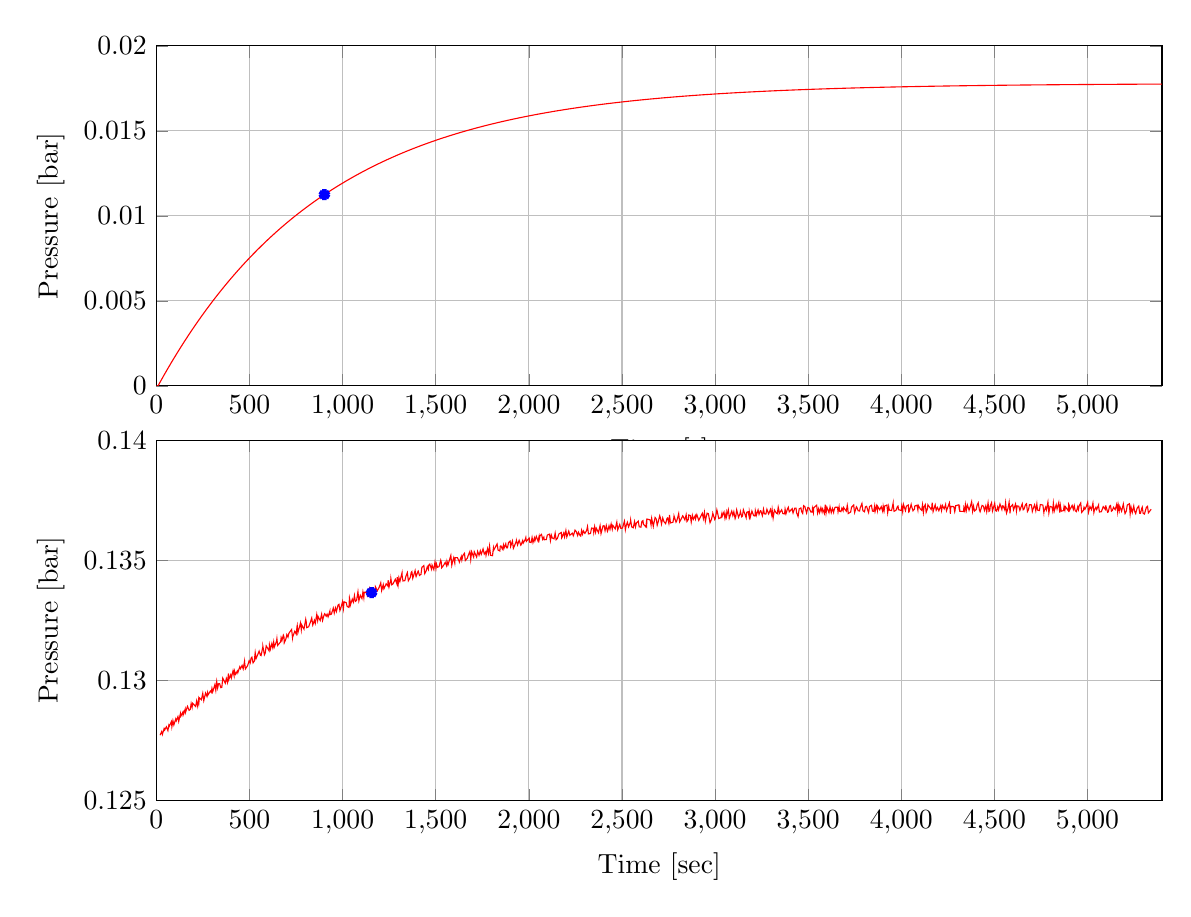
\begin{tikzpicture}

\begin{axis}[%
scaled y ticks = false,
 y tick label style={/pgf/number format/fixed,
/pgf/number format/1000 sep = \thinspace}, % Optional if you want to replace comma as the 1000 separator 
width=5.028in,
height=1.7in,
at={(0.758in,2.554in)},
scale only axis,
xmin=0,
xmax=5400,
xlabel style={font=\color{black}},
xlabel={Time [s]},
ymin=0,
ymax=0.02,
yticklabel style={/pgf/number format/.cd,fixed,precision=3},
ylabel style={font=\color{black}},
ylabel={Pressure [bar]},
axis background/.style={fill=white},
xmajorgrids,
ymajorgrids,
legend style={legend cell align=left, align=left, draw=black}
]
\addplot [color=red,solid,forget plot]
  table[row sep=crcr]{%
0	0\\
8.93323388268949	0\\
17.866467765379	0.000177027924568163\\
26.7997016480685	0.000352294391588673\\
35.732935530758	0.000525816927859629\\
44.6661694134474	0.000697612885784553\\
53.5994032961369	0.000867699445107638\\
62.5326371788264	0.00103609361463174\\
71.4658710615159	0.00120281223391928\\
80.3991049442054	0.00136787197497619\\
89.3323388268949	0.00153128934391917\\
98.2655727095844	0.00169308068262627\\
107.198806592274	0.00185326217037112\\
116.132040474963	0.00201184982544087\\
125.065274357653	0.00216885950673801\\
133.998508240342	0.00232430691536631\\
142.931742123032	0.0024782075962009\\
151.864976005721	0.00263057693944281\\
160.798209888411	0.00278143018215799\\
169.7314437711	0.00293078240980101\\
178.66467765379	0.00307864855772366\\
187.597911536479	0.00322504341266846\\
196.531145419169	0.00336998161424736\\
205.464379301858	0.00351347765640572\\
214.397613184548	0.00365554588887171\\
223.330847067237	0.0037962005185913\\
232.264080949927	0.00393545561114897\\
241.197314832616	0.00407332509217425\\
250.130548715306	0.00420982274873435\\
259.063782597995	0.00434496223071284\\
267.997016480685	0.00447875705217464\\
276.930250363374	0.00461122059271748\\
285.863484246064	0.00474236609880983\\
294.796718128753	0.00487220668511561\\
303.729952011443	0.00500075533580558\\
312.663185894132	0.00512802490585587\\
321.596419776822	0.00525402812233342\\
330.529653659511	0.00537877758566872\\
339.462887542201	0.00550228577091587\\
348.39612142489	0.00562456502900008\\
357.32935530758	0.00574562758795279\\
366.262589190269	0.00586548555413446\\
375.195823072959	0.00598415091344526\\
384.129056955648	0.00610163553252361\\
393.062290838338	0.00621795115993292\\
401.995524721027	0.0063331094273364\\
410.928758603717	0.00644712185066027\\
419.861992486406	0.00655999983124534\\
428.795226369095	0.00667175465698718\\
437.728460251785	0.00678239750346491\\
446.661694134474	0.00689193943505874\\
455.594928017164	0.00700039140605645\\
464.528161899853	0.00710776426174885\\
473.461395782543	0.00721406873951423\\
482.394629665232	0.00731931546989221\\
491.327863547922	0.00742351497764674\\
500.261097430611	0.00752667768281861\\
509.194331313301	0.00762881390176744\\
518.12756519599	0.00772993384820337\\
527.06079907868	0.00783004763420837\\
535.994032961369	0.00792916527124754\\
544.927266844059	0.0080272966711702\\
553.860500726748	0.0081244516472011\\
562.793734609438	0.00822063991492178\\
571.726968492127	0.0083158710932421\\
580.660202374817	0.00841015470536215\\
589.593436257506	0.00850350017972459\\
598.526670140196	0.00859591685095749\\
607.459904022885	0.0086874139608078\\
616.393137905575	0.00877800065906555\\
625.326371788264	0.00886768600447881\\
634.259605670954	0.0089564789656596\\
643.192839553643	0.00904438842198073\\
652.126073436333	0.00913142316446378\\
661.059307319022	0.00921759189665818\\
669.992541201712	0.00930290323551158\\
678.925775084401	0.00938736571223156\\
687.859008967091	0.00947098777313875\\
696.79224284978	0.00955377778051148\\
705.72547673247	0.009635744013422\\
714.658710615159	0.00971689466856441\\
723.591944497849	0.00979723786107432\\
732.525178380538	0.00987678162534038\\
741.458412263228	0.00995553391580774\\
750.391646145917	0.0100335026077735\\
759.324880028607	0.0101106954981741\\
768.258113911296	0.0101871203063654\\
777.191347793986	0.0102627846748941\\
786.124581676675	0.0103376961702625\\
795.057815559364	0.0104118622836849\\
803.991049442054	0.0104852904318366\\
812.924283324744	0.0105579879575959\\
821.857517207433	0.0106299621307782\\
830.790751090123	0.0107012201488629\\
839.723984972812	0.0107717691377134\\
848.657218855501	0.0108416161522896\\
857.590452738191	0.0109107681773531\\
866.52368662088	0.0109792321281664\\
875.45692050357	0.0110470148511836\\
884.390154386259	0.0111141231247355\\
893.323388268949	0.0111805636597075\\
902.256622151638	0.0112463431002104\\
911.189856034328	0.0113114680242452\\
920.123089917017	0.0113759449443605\\
929.056323799707	0.011439780308304\\
937.989557682396	0.0115029804996673\\
946.922791565086	0.011565551838524\\
955.856025447775	0.0116275005820621\\
964.789259330465	0.0116888329252095\\
973.722493213154	0.0117495550012535\\
982.655727095844	0.0118096728824541\\
991.588960978533	0.0118691925806514\\
1000.52219486122	0.0119281200478666\\
1009.45542874391	0.0119864611768973\\
1018.3886626266	0.0120442218019068\\
1027.32189650929	0.0121014076990077\\
1036.25513039198	0.0121580245868388\\
1045.18836427467	0.012214078127138\\
1054.12159815736	0.0122695739253076\\
1063.05483204005	0.0123245175309755\\
1071.98806592274	0.0123789144385497\\
1080.92129980543	0.0124327700877679\\
1089.85453368812	0.0124860898642415\\
1098.78776757081	0.0125388790999943\\
1107.7210014535	0.0125911430739954\\
1116.65423533619	0.0126428870126875\\
1125.58746921888	0.0126941160905089\\
1134.52070310157	0.0127448354304119\\
1143.45393698425	0.0127950501043741\\
1152.38717086694	0.0128447651339065\\
1161.32040474963	0.0128939854905547\\
1170.25363863232	0.0129427160963971\\
1179.18687251501	0.0129909618245364\\
1188.1201063977	0.0130387274995869\\
1197.05334028039	0.0130860178981576\\
1205.98657416308	0.013132837749329\\
1214.91980804577	0.0131791917351267\\
1223.85304192846	0.0132250844909895\\
1232.78627581115	0.0132705206062324\\
1241.71950969384	0.0133155046245063\\
1250.65274357653	0.0133600410442519\\
1259.58597745922	0.0134041343191495\\
1268.51921134191	0.0134477888585649\\
1277.4524452246	0.0134910090279896\\
1286.38567910729	0.0135337991494778\\
1295.31891298998	0.0135761635020788\\
1304.25214687267	0.0136181063222644\\
1313.18538075535	0.0136596318043528\\
1322.11861463804	0.0137007441009282\\
1331.05184852073	0.0137414473232556\\
1339.98508240342	0.0137817455416924\\
1348.91831628611	0.0138216427860954\\
1357.8515501688	0.0138611430462234\\
1366.78478405149	0.0139002502721366\\
1375.71801793418	0.0139389683745913\\
1384.65125181687	0.0139773012254313\\
1393.58448569956	0.0140152526579747\\
1402.51771958225	0.0140528264673975\\
1411.45095346494	0.0140900264111132\\
1420.38418734763	0.0141268562091483\\
1429.31742123032	0.0141633195445143\\
1438.25065511301	0.0141994200635764\\
1447.1838889957	0.0142351613764175\\
1456.11712287839	0.0142705470572\\
1465.05035676108	0.0143055806445223\\
1473.98359064377	0.0143402656417736\\
1482.91682452646	0.0143746055174835\\
1491.85005840914	0.0144086037056692\\
1500.78329229183	0.0144422636061789\\
1509.71652617452	0.0144755885850317\\
1518.64976005721	0.0145085819747544\\
1527.5829939399	0.0145412470747144\\
1536.51622782259	0.0145735871514498\\
1545.44946170528	0.0146056054389964\\
1554.38269558797	0.0146373051392105\\
1563.31592947066	0.0146686894220895\\
1572.24916335335	0.0146997614260889\\
1581.18239723604	0.0147305242584358\\
1590.11563111873	0.0147609809954401\\
1599.04886500142	0.0147911346828018\\
1607.98209888411	0.0148209883359156\\
1616.9153327668	0.0148505449401728\\
1625.84856664949	0.0148798074512591\\
1634.78180053218	0.0149087787954511\\
1643.71503441487	0.0149374618699081\\
1652.64826829756	0.0149658595429624\\
1661.58150218025	0.0149939746544058\\
1670.51473606293	0.0150218100157738\\
1679.44796994562	0.0150493684106265\\
1688.38120382831	0.0150766525948272\\
1697.314437711	0.0151036652968179\\
1706.24767159369	0.0151304092178922\\
1715.18090547638	0.0151568870324652\\
1724.11413935907	0.0151831013883413\\
1733.04737324176	0.0152090549069787\\
1741.98060712445	0.0152347501837517\\
1750.91384100714	0.0152601897882102\\
1759.84707488983	0.0152853762643365\\
1768.78030877252	0.0153103121308001\\
1777.71354265521	0.0153349998812092\\
1786.6467765379	0.0153594419843601\\
1795.58001042059	0.0153836408844842\\
1804.51324430328	0.0154075990014925\\
1813.44647818597	0.0154313187312174\\
1822.37971206866	0.0154548024456522\\
1831.31294595135	0.0154780524931888\\
1840.24617983403	0.015501071198852\\
1849.17941371672	0.0155238608645322\\
1858.11264759941	0.0155464237692157\\
1867.0458814821	0.0155687621692125\\
1875.97911536479	0.0155908782983818\\
1884.91234924748	0.0156127743683556\\
1893.84558313017	0.01563445256876\\
1902.77881701286	0.0156559150674335\\
1911.71205089555	0.0156771640106448\\
1920.64528477824	0.0156982015233063\\
1929.57851866093	0.0157190297091876\\
1938.51175254362	0.0157396506511253\\
1947.44498642631	0.0157600664112313\\
1956.378220309	0.0157802790310993\\
1965.31145419169	0.0158002905320088\\
1974.24468807438	0.0158201029151271\\
1983.17792195707	0.0158397181617096\\
1992.11115583976	0.015859138233298\\
2001.04438972245	0.0158783650719162\\
2009.97762360514	0.0158974006002646\\
2018.91085748782	0.0159162467219125\\
2027.84409137051	0.0159349053214885\\
2036.7773252532	0.0159533782648684\\
2045.71055913589	0.0159716673993628\\
2054.64379301858	0.0159897745539007\\
2063.57702690127	0.0160077015392133\\
2072.51026078396	0.0160254501480147\\
2081.44349466665	0.0160430221551809\\
2090.37672854934	0.016060419317928\\
2099.30996243203	0.0160776433759872\\
2108.24319631472	0.0160946960517792\\
2117.17643019741	0.0161115790505863\\
2126.1096640801	0.0161282940607229\\
2135.04289796279	0.0161448427537047\\
2143.97613184548	0.016161226784415\\
2152.90936572817	0.0161774477912712\\
2161.84259961086	0.0161935073963879\\
2170.77583349355	0.0162094072057395\\
2179.70906737624	0.0162251488093208\\
2188.64230125892	0.0162407337813056\\
2197.57553514161	0.0162561636802046\\
2206.5087690243	0.0162714400490211\\
2215.44200290699	0.0162865644154051\\
2224.37523678968	0.0163015382918063\\
2233.30847067237	0.0163163631756253\\
2242.24170455506	0.0163310405493632\\
2251.17493843775	0.0163455718807702\\
2260.10817232044	0.0163599586229919\\
2269.04140620313	0.016374202214715\\
2277.97464008582	0.016388304080311\\
2286.90787396851	0.0164022656299785\\
2295.8411078512	0.0164160882598847\\
2304.77434173389	0.0164297733523044\\
2313.70757561658	0.0164433222757587\\
2322.64080949927	0.0164567363851516\\
2331.57404338196	0.0164700170219058\\
2340.50727726465	0.0164831655140963\\
2349.44051114734	0.0164961831765837\\
2358.37374503003	0.0165090713111456\\
2367.30697891271	0.0165218312066064\\
2376.2402127954	0.0165344641389668\\
2385.17344667809	0.0165469713715309\\
2394.10668056078	0.0165593541550328\\
2403.03991444347	0.0165716137277614\\
2411.97314832616	0.0165837513156848\\
2420.90638220885	0.0165957681325722\\
2429.83961609154	0.0166076653801155\\
2438.77284997423	0.01661944424805\\
2447.70608385692	0.0166311059142724\\
2456.63931773961	0.0166426515449596\\
2465.5725516223	0.0166540822946846\\
2474.50578550499	0.0166653993065321\\
2483.43901938768	0.0166766037122133\\
2492.37225327037	0.0166876966321783\\
2501.30548715306	0.0166986791757286\\
2510.23872103575	0.0167095524411282\\
2519.17195491844	0.016720317515713\\
2528.10518880113	0.0167309754759997\\
2537.03842268382	0.0167415273877936\\
2545.9716565665	0.016751974306295\\
2554.90489044919	0.0167623172762047\\
2563.83812433188	0.0167725573318286\\
2572.77135821457	0.0167826954971812\\
2581.70459209726	0.0167927327860878\\
2590.63782597995	0.0168026702022859\\
2599.57105986264	0.0168125087395257\\
2608.50429374533	0.0168222493816695\\
2617.43752762802	0.0168318931027899\\
2626.37076151071	0.0168414408672673\\
2635.3039953934	0.0168508936298864\\
2644.23722927609	0.0168602523359316\\
2653.17046315878	0.0168695179212817\\
2662.10369704147	0.0168786913125032\\
2671.03693092416	0.016887773426943\\
2679.97016480685	0.0168967651728206\\
2688.90339868954	0.0169056674493182\\
2697.83663257223	0.0169144811466713\\
2706.76986645492	0.0169232071462571\\
2715.7031003376	0.0169318463206831\\
2724.63633422029	0.0169403995338743\\
2733.56956810298	0.0169488676411594\\
2742.50280198567	0.0169572514893563\\
2751.43603586836	0.0169655519168573\\
2760.36926975105	0.0169737697537121\\
2769.30250363374	0.0169819058217116\\
2778.23573751643	0.0169899609344696\\
2787.16897139912	0.0169979358975043\\
2796.10220528181	0.0170058315083189\\
2805.0354391645	0.0170136485564814\\
2813.96867304719	0.0170213878237032\\
2822.90190692988	0.0170290500839179\\
2831.83514081257	0.017036636103358\\
2840.76837469526	0.0170441466406321\\
2849.70160857795	0.0170515824468003\\
2858.63484246064	0.0170589442654497\\
2867.56807634333	0.0170662328327685\\
2876.50131022602	0.0170734488776198\\
2885.4345441087	0.0170805931216142\\
2894.36777799139	0.0170876662791824\\
2903.30101187408	0.0170946690576462\\
2912.23424575677	0.0171016021572894\\
2921.16747963946	0.0171084662714282\\
2930.10071352215	0.0171152620864797\\
2939.03394740484	0.0171219902820314\\
2947.96718128753	0.0171286515309086\\
2956.90041517022	0.017135246499242\\
2965.83364905291	0.0171417758465342\\
2974.7668829356	0.0171482402257254\\
2983.70011681829	0.0171546402832592\\
2992.63335070098	0.0171609766591468\\
3001.56658458367	0.0171672499870314\\
3010.49981846636	0.0171734608942511\\
3019.43305234905	0.0171796100019021\\
3028.36628623174	0.0171856979249003\\
3037.29952011443	0.0171917252720434\\
3046.23275399712	0.0171976926460713\\
3055.16598787981	0.0172036006437265\\
3064.09922176249	0.0172094498558139\\
3073.03245564518	0.0172152408672598\\
3081.96568952787	0.0172209742571703\\
3090.89892341056	0.0172266505988893\\
3099.83215729325	0.017232270460056\\
3108.76539117594	0.0172378344026613\\
3117.69862505863	0.0172433429831043\\
3126.63185894132	0.0172487967522477\\
3135.56509282401	0.0172541962554732\\
3144.4983267067	0.0172595420327358\\
3153.43156058939	0.0172648346186179\\
3162.36479447208	0.0172700745423825\\
3171.29802835477	0.0172752623280267\\
3180.23126223746	0.0172803984943333\\
3189.16449612015	0.0172854835549236\\
3198.09773000284	0.0172905180183079\\
3207.03096388553	0.017295502387937\\
3215.96419776822	0.0173004371622521\\
3224.89743165091	0.0173053228347349\\
3233.8306655336	0.0173101598939569\\
3242.76389941628	0.0173149488236281\\
3251.69713329897	0.0173196901026457\\
3260.63036718166	0.0173243842051417\\
3269.56360106435	0.0173290316005304\\
3278.49683494704	0.0173336327535553\\
3287.43006882973	0.0173381881243358\\
3296.36330271242	0.0173426981684127\\
3305.29653659511	0.0173471633367945\\
3314.2297704778	0.0173515840760018\\
3323.16300436049	0.0173559608281124\\
3332.09623824318	0.0173602940308053\\
3341.02947212587	0.0173645841174044\\
3349.96270600856	0.0173688315169221\\
3358.89593989125	0.0173730366541021\\
3367.82917377394	0.0173771999494617\\
3376.76240765663	0.017381321819334\\
3385.69564153932	0.0173854026759096\\
3394.62887542201	0.0173894429272777\\
3403.5621093047	0.0173934429774669\\
3412.49534318738	0.0173974032264857\\
3421.42857707007	0.0174013240703623\\
3430.36181095276	0.0174052059011846\\
3439.29504483545	0.017409049107139\\
3448.22827871814	0.0174128540725495\\
3457.16151260083	0.0174166211779157\\
3466.09474648352	0.0174203507999517\\
3475.02798036621	0.0174240433116226\\
3483.9612142489	0.017427699082183\\
3492.89444813159	0.0174313184772131\\
3501.82768201428	0.0174349018586553\\
3510.76091589697	0.0174384495848511\\
3519.69414977966	0.0174419620105761\\
3528.62738366235	0.0174454394870759\\
3537.56061754504	0.0174488823621011\\
3546.49385142773	0.0174522909799422\\
3555.42708531042	0.017455665681464\\
3564.36031919311	0.0174590068041395\\
3573.2935530758	0.0174623146820839\\
3582.22678695849	0.0174655896460878\\
3591.16002084117	0.0174688320236504\\
3600.09325472386	0.0174720421390124\\
3609.02648860655	0.017475220313188\\
3617.95972248924	0.0174783668639973\\
3626.89295637193	0.0174814821060983\\
3635.82619025462	0.0174845663510177\\
3644.75942413731	0.0174876199071828\\
3653.69265802	0.0174906430799517\\
3662.62589190269	0.0174936361716445\\
3671.55912578538	0.0174965994815728\\
3680.49235966807	0.0174995333060701\\
3689.42559355076	0.0175024379385216\\
3698.35882743345	0.0175053136693928\\
3707.29206131614	0.0175081607862595\\
3716.22529519883	0.0175109795738357\\
3725.15852908152	0.0175137703140027\\
3734.09176296421	0.0175165332858368\\
3743.0249968469	0.0175192687656376\\
3751.95823072959	0.0175219770269555\\
3760.89146461227	0.017524658340619\\
3769.82469849496	0.0175273129747617\\
3778.75793237765	0.0175299411948494\\
3787.69116626034	0.0175325432637062\\
3796.62440014303	0.0175351194415414\\
3805.55763402572	0.017537669985975\\
3814.49086790841	0.0175401951520636\\
3823.4241017911	0.0175426951923259\\
3832.35733567379	0.0175451703567683\\
3841.29056955648	0.0175476208929092\\
3850.22380343917	0.0175500470458044\\
3859.15703732186	0.0175524490580713\\
3868.09027120455	0.0175548271699132\\
3877.02350508724	0.0175571816191433\\
3885.95673896993	0.0175595126412086\\
3894.88997285262	0.0175618204692133\\
3903.82320673531	0.0175641053339422\\
3912.756440618	0.0175663674638837\\
3921.68967450069	0.0175686070852528\\
3930.62290838338	0.0175708244220135\\
3939.55614226606	0.0175730196959015\\
3948.48937614875	0.0175751931264461\\
3957.42261003144	0.0175773449309921\\
3966.35584391413	0.0175794753247219\\
3975.28907779682	0.0175815845206767\\
3984.22231167951	0.0175836727297779\\
3993.1555455622	0.0175857401608482\\
4002.08877944489	0.0175877870206325\\
4011.02201332758	0.0175898135138186\\
4019.95524721027	0.0175918198430576\\
4028.88848109296	0.017593806208984\\
4037.82171497565	0.0175957728102362\\
4046.75494885834	0.0175977198434761\\
4055.68818274103	0.0175996475034085\\
4064.62141662372	0.0176015559828013\\
4073.55465050641	0.017603445472504\\
4082.4878843891	0.0176053161614671\\
4091.42111827179	0.0176071682367612\\
4100.35435215448	0.0176090018835954\\
4109.28758603717	0.017610817285336\\
4118.22081991985	0.0176126146235248\\
4127.15405380254	0.017614394077897\\
4136.08728768523	0.0176161558263998\\
4145.02052156792	0.0176179000452093\\
4153.95375545061	0.0176196269087491\\
4162.8869893333	0.017621336589707\\
4171.82022321599	0.0176230292590525\\
4180.75345709868	0.0176247050860541\\
4189.68669098137	0.0176263642382959\\
4198.61992486406	0.0176280068816946\\
4207.55315874675	0.0176296331805158\\
4216.48639262944	0.017631243297391\\
4225.41962651213	0.0176328373933331\\
4234.35286039482	0.0176344156277532\\
4243.28609427751	0.017635978158476\\
4252.2193281602	0.017637525141756\\
4261.15256204289	0.0176390567322929\\
4270.08579592558	0.017640573083247\\
4279.01902980827	0.0176420743462547\\
4287.95226369096	0.0176435606714436\\
4296.88549757364	0.0176450322074475\\
4305.81873145633	0.0176464891014214\\
4314.75196533902	0.0176479314990558\\
4323.68519922171	0.0176493595445917\\
4332.6184331044	0.017650773380835\\
4341.55166698709	0.0176521731491705\\
4350.48490086978	0.0176535589895763\\
4359.41813475247	0.0176549310406375\\
4368.35136863516	0.0176562894395604\\
4377.28460251785	0.0176576343221863\\
4386.21783640054	0.0176589658230043\\
4395.15107028323	0.0176602840751659\\
4404.08430416592	0.0176615892104973\\
4413.01753804861	0.0176628813595132\\
4421.9507719313	0.0176641606514296\\
4430.88400581399	0.0176654272141768\\
4439.81723969668	0.0176666811744122\\
4448.75047357937	0.0176679226575329\\
4457.68370746206	0.0176691517876883\\
4466.61694134474	0.0176703686877925\\
4475.55017522743	0.0176715734795364\\
4484.48340911012	0.0176727662834004\\
4493.41664299281	0.0176739472186659\\
4502.3498768755	0.0176751164034273\\
4511.28311075819	0.0176762739546042\\
4520.21634464088	0.0176774199879527\\
4529.14957852357	0.0176785546180772\\
4538.08281240626	0.0176796779584415\\
4547.01604628895	0.0176807901213808\\
4555.94928017164	0.0176818912181123\\
4564.88251405433	0.0176829813587465\\
4573.81574793702	0.0176840606522986\\
4582.74898181971	0.0176851292066988\\
4591.6822157024	0.0176861871288034\\
4600.61544958509	0.0176872345244056\\
4609.54868346778	0.0176882714982459\\
4618.48191735047	0.0176892981540224\\
4627.41515123316	0.0176903145944018\\
4636.34838511584	0.0176913209210289\\
4645.28161899853	0.0176923172345372\\
4654.21485288122	0.017693303634559\\
4663.14808676391	0.017694280219735\\
4672.0813206466	0.0176952470877248\\
4681.01455452929	0.0176962043352158\\
4689.94778841198	0.0176971520579337\\
4698.88102229467	0.0176980903506516\\
4707.81425617736	0.0176990193071995\\
4716.74749006005	0.017699939020474\\
4725.68072394274	0.017700849582447\\
4734.61395782543	0.0177017510841757\\
4743.54719170812	0.0177026436158109\\
4752.48042559081	0.0177035272666067\\
4761.4136594735	0.0177044021249287\\
4770.34689335619	0.0177052682782638\\
4779.28012723888	0.0177061258132278\\
4788.21336112157	0.017706974815575\\
4797.14659500426	0.0177078153702065\\
4806.07982888695	0.0177086475611784\\
4815.01306276963	0.0177094714717105\\
4823.94629665232	0.0177102871841946\\
4832.87953053501	0.0177110947802026\\
4841.8127644177	0.0177118943404949\\
4850.74599830039	0.0177126859450282\\
4859.67923218308	0.0177134696729635\\
4868.61246606577	0.0177142456026744\\
4877.54569994846	0.0177150138117545\\
4886.47893383115	0.0177157743770253\\
4895.41216771384	0.0177165273745442\\
4904.34540159653	0.0177172728796114\\
4913.27863547922	0.0177180109667781\\
4922.21186936191	0.0177187417098537\\
4931.1451032446	0.0177194651819131\\
4940.07833712729	0.0177201814553041\\
4949.01157100998	0.0177208906016548\\
4957.94480489267	0.0177215926918802\\
4966.87803877536	0.0177222877961902\\
4975.81127265805	0.0177229759840957\\
4984.74450654073	0.017723657324416\\
4993.67774042342	0.0177243318852859\\
5002.61097430611	0.0177249997341619\\
5011.5442081888	0.0177256609378296\\
5020.47744207149	0.0177263155624098\\
5029.41067595418	0.0177269636733657\\
5038.34390983687	0.0177276053355089\\
5047.27714371956	0.017728240613006\\
5056.21037760225	0.0177288695693855\\
5065.14361148494	0.0177294922675435\\
5074.07684536763	0.0177301087697504\\
5083.01007925032	0.0177307191376569\\
5091.94331313301	0.0177313234323003\\
5100.8765470157	0.0177319217141106\\
5109.80978089839	0.0177325140429166\\
5118.74301478108	0.0177331004779516\\
5127.67624866377	0.0177336810778596\\
5136.60948254646	0.0177342559007011\\
5145.54271642915	0.0177348250039589\\
5154.47595031183	0.0177353884445438\\
5163.40918419452	0.0177359462788004\\
5172.34241807721	0.0177364985625125\\
5181.2756519599	0.0177370453509091\\
5190.20888584259	0.0177375866986693\\
5199.14211972528	0.0177381226599286\\
5208.07535360797	0.0177386532882834\\
5217.00858749066	0.0177391786367971\\
5225.94182137335	0.0177396987580049\\
5234.87505525604	0.0177402137039194\\
5243.80828913873	0.0177407235260357\\
5252.74152302142	0.0177412282753364\\
5261.67475690411	0.0177417280022969\\
5270.6079907868	0.0177422227568903\\
5279.54122466949	0.0177427125885925\\
5288.47445855218	0.0177431975463871\\
5297.40769243487	0.0177436776787703\\
5306.34092631756	0.0177441530337557\\
5315.27416020025	0.0177446236588793\\
5324.20739408294	0.0177450896012039\\
5333.14062796562	0.0177455509073243\\
5342.07386184831	0.0177460076233713\\
5351.007095731	0.0177464597950171\\
5359.94032961369	0.0177469074674791\\
5368.87356349638	0.0177473506855251\\
5377.80679737907	0.0177477894934771\\
5386.74003126176	0.0177482239352164\\
5395.67326514445	0.0177486540541875\\
5404.60649902714	0.0177490798934027\\
5413.53973290983	0.0177495014954462\\
5422.47296679252	0.0177499189024787\\
5431.40620067521	0.0177503321562412\\
5440.3394345579	0.0177507412980594\\
5449.27266844059	0.0177511463688479\\
5458.20590232328	0.0177515474091141\\
5467.13913620597	0.0177519444589624\\
5476.07237008866	0.0177523375580981\\
5485.00560397135	0.0177527267458314\\
5493.93883785404	0.0177531120610815\\
5502.87207173673	0.0177534935423802\\
5511.80530561941	0.017753871227876\\
5520.7385395021	0.0177542451553377\\
5529.67177338479	0.0177546153621585\\
5538.60500726748	0.0177549818853593\\
5547.53824115017	0.0177553447615928\\
5556.47147503286	0.0177557040271468\\
5565.40470891555	0.0177560597179484\\
5574.33794279824	0.0177564118695667\\
5583.27117668093	0.0177567605172174\\
5592.20441056362	0.0177571056957655\\
5601.13764444631	0.0177574474397292\\
5610.070878329	0.017757785783283\\
5619.00411221169	0.0177581207602618\\
5627.93734609438	0.0177584524041634\\
5636.87057997707	0.0177587807481525\\
5645.80381385976	0.0177591058250639\\
5654.73704774245	0.0177594276674055\\
5663.67028162514	0.0177597463073618\\
5672.60351550783	0.017760061776797\\
5681.53674939052	0.0177603741072585\\
5690.4699832732	0.0177606833299795\\
5699.40321715589	0.0177609894758825\\
5708.33645103858	0.0177612925755824\\
5717.26968492127	0.0177615926593895\\
5726.20291880396	0.0177618897573123\\
5735.13615268665	0.017762183899061\\
5744.06938656934	0.0177624751140499\\
5753.00262045203	0.0177627634314008\\
5761.93585433472	0.0177630488799457\\
5770.86908821741	0.0177633314882297\\
5779.8023221001	0.0177636112845139\\
5788.73555598279	0.0177638882967781\\
5797.66878986548	0.0177641625527238\\
5806.60202374817	0.0177644340797769\\
5815.53525763086	0.0177647029050902\\
5824.46849151355	0.0177649690555465\\
5833.40172539624	0.0177652325577612\\
5842.33495927893	0.0177654934380846\\
5851.26819316162	0.017765751722605\\
5860.20142704431	0.0177660074371511\\
5869.13466092699	0.0177662606072946\\
5878.06789480968	0.0177665112583527\\
5887.00112869237	0.0177667594153907\\
5895.93436257506	0.0177670051032246\\
5904.86759645775	0.0177672483464233\\
5913.80083034044	0.0177674891693113\\
5922.73406422313	0.0177677275959713\\
5931.66729810582	0.0177679636502459\\
5940.60053198851	0.0177681973557409\\
5949.5337658712	0.0177684287358271\\
5958.46699975389	0.0177686578136425\\
5967.40023363658	0.0177688846120953\\
5976.33346751927	0.0177691091538654\\
5985.26670140196	0.0177693314614073\\
5994.19993528465	0.0177695515569518\\
6003.13316916734	0.0177697694625087\\
6012.06640305003	0.0177699851998688\\
6020.99963693272	0.0177701987906059\\
6029.93287081541	0.0177704102560794\\
6038.86610469809	0.0177706196174359\\
6047.79933858078	0.0177708268956118\\
6056.73257246347	0.0177710321113351\\
6065.66580634616	0.0177712352851275\\
6074.59904022885	0.0177714364373066\\
6083.53227411154	0.0177716355879878\\
6092.46550799423	0.0177718327570863\\
6101.39874187692	0.0177720279643192\\
6110.33197575961	0.0177722212292073\\
6119.2652096423	0.0177724125710774\\
6128.19844352499	0.0177726020090638\\
6137.13167740768	0.0177727895621105\\
6146.06491129037	0.0177729752489729\\
6154.99814517306	0.0177731590882198\\
6163.93137905575	0.0177733410982354\\
6172.86461293844	0.0177735212972208\\
6181.79784682113	0.0177736997031961\\
6190.73108070382	0.017773876334002\\
6199.66431458651	0.0177740512073017\\
6208.5975484692	0.0177742243405828\\
6217.53078235188	0.0177743957511587\\
6226.46401623457	0.0177745654561705\\
6235.39725011726	0.0177747334725891\\
6244.33048399995	0.0177748998172161\\
6253.26371788264	0.0177750645066862\\
6262.19695176533	0.0177752275574684\\
6271.13018564802	0.0177753889858679\\
6280.06341953071	0.0177755488080278\\
6288.9966534134	0.0177757070399304\\
6297.92988729609	0.0177758636973991\\
6306.86312117878	0.0177760187960996\\
6315.79635506147	0.0177761723515421\\
6324.72958894416	0.0177763243790821\\
6333.66282282685	0.0177764748939226\\
6342.59605670954	0.0177766239111152\\
6351.52929059223	0.0177767714455617\\
6360.46252447492	0.0177769175120157\\
6369.39575835761	0.0177770621250841\\
6378.3289922403	0.0177772052992281\\
6387.26222612298	0.0177773470487654\\
6396.19546000567	0.0177774873878709\\
6405.12869388836	0.0177776263305789\\
6414.06192777105	0.0177777638907836\\
6422.99516165374	0.0177779000822412\\
6431.92839553643	0.0177780349185709\\
6440.86162941912	0.0177781684132565\\
6449.79486330181	0.0177783005796477\\
6458.7280971845	0.017778431430961\\
6467.66133106719	0.0177785609802818\\
6476.59456494988	0.0177786892405652\\
6485.52779883257	0.0177788162246372\\
6494.46103271526	0.0177789419451964\\
6503.39426659795	0.017779066414815\\
6512.32750048064	0.0177791896459399\\
6521.26073436333	0.0177793116508945\\
6530.19396824602	0.0177794324418794\\
6539.12720212871	0.0177795520309736\\
6548.0604360114	0.0177796704301363\\
6556.99366989408	0.0177797876512075\\
6565.92690377677	0.0177799037059094\\
6574.86013765946	0.0177800186058475\\
6583.79337154215	0.0177801323625119\\
6592.72660542484	0.0177802449872785\\
6601.65983930753	0.0177803564914097\\
6610.59307319022	0.0177804668860561\\
6619.52630707291	0.0177805761822573\\
6628.4595409556	0.0177806843909429\\
6637.39277483829	0.017780791522934\\
6646.32600872098	0.0177808975889438\\
6655.25924260367	0.0177810025995789\\
6664.19247648636	0.0177811065653407\\
6673.12571036905	0.0177812094966257\\
6682.05894425174	0.0177813114037271\\
6690.99217813443	0.0177814122968358\\
6699.92541201712	0.0177815121860411\\
6708.85864589981	0.017781611081332\\
6717.7918797825	0.0177817089925982\\
6726.72511366518	0.0177818059296309\\
6735.65834754787	0.0177819019021239\\
6744.59158143056	0.0177819969196745\\
6753.52481531325	0.0177820909917845\\
6762.45804919594	0.0177821841278612\\
6771.39128307863	0.0177822763372183\\
6780.32451696132	0.0177823676290768\\
6789.25775084401	0.0177824580125661\\
6798.1909847267	0.0177825474967244\\
6807.12421860939	0.0177826360905004\\
6816.05745249208	0.0177827238027535\\
6824.99068637477	0.0177828106422549\\
6833.92392025746	0.0177828966176887\\
6842.85715414015	0.0177829817376525\\
6851.79038802284	0.0177830660106584\\
6860.72362190553	0.0177831494451337\\
6869.65685578822	0.017783232049422\\
6878.59008967091	0.0177833138317838\\
6887.5233235536	0.0177833948003974\\
6896.45655743629	0.0177834749633597\\
6905.38979131897	0.0177835543286871\\
6914.32302520166	0.0177836329043161\\
6923.25625908435	0.0177837106981045\\
6932.18949296704	0.0177837877178316\\
6941.12272684973	0.0177838639711995\\
6950.05596073242	0.0177839394658336\\
6958.98919461511	0.0177840142092834\\
6967.9224284978	0.0177840882090233\\
6976.85566238049	0.0177841614724535\\
6985.78889626318	0.0177842340069002\\
6994.72213014587	0.017784305819617\\
7003.65536402856	0.0177843769177852\\
7012.58859791125	0.0177844473085147\\
7021.52183179394	0.0177845169988447\\
7030.45506567663	0.0177845859957441\\
7039.38829955932	0.0177846543061129\\
7048.32153344201	0.017784721936782\\
7057.2547673247	0.0177847888945146\\
7066.18800120739	0.0177848551860066\\
7075.12123509008	0.017784920817887\\
7084.05446897276	0.0177849857967193\\
7092.98770285545	0.0177850501290013\\
7101.92093673814	0.0177851138211663\\
7110.85417062083	0.0177851768795835\\
7119.78740450352	0.0177852393105589\\
7128.72063838621	0.0177853011203357\\
7137.6538722689	0.0177853623150948\\
7146.58710615159	0.0177854229009558\\
7155.52034003428	0.0177854828839772\\
7164.45357391697	0.0177855422701576\\
7173.38680779966	0.0177856010654355\\
7182.32004168235	0.0177856592756906\\
7191.25327556504	0.0177857169067438\\
7200.18650944773	0.0177857739643584\\
7209.11974333042	0.0177858304542401\\
7218.05297721311	0.0177858863820381\\
7226.9862110958	0.017785941753345\\
7235.91944497849	0.0177859965736982\\
7244.85267886118	0.0177860508485797\\
7253.78591274387	0.017786104583417\\
7262.71914662655	0.0177861577835836\\
7271.65238050924	0.0177862104543997\\
7280.58561439193	0.0177862626011323\\
7289.51884827462	0.0177863142289962\\
7298.45208215731	0.0177863653431541\\
7307.38531604	0.0177864159487177\\
7316.31854992269	0.0177864660507473\\
7325.25178380538	0.0177865156542534\\
7334.18501768807	0.0177865647641963\\
7343.11825157076	0.017786613385487\\
7352.05148545345	0.0177866615229877\\
7360.98471933614	0.0177867091815121\\
7369.91795321883	0.0177867563658263\\
7378.85118710152	0.0177868030806486\\
7387.78442098421	0.0177868493306507\\
7396.7176548669	0.0177868951204574\\
7405.65088874959	0.0177869404546479\\
7414.58412263228	0.0177869853377555\\
7423.51735651497	0.0177870297742688\\
7432.45059039766	0.0177870737686312\\
7441.38382428034	0.0177871173252424\\
7450.31705816303	0.017787160448458\\
7459.25029204572	0.0177872031425904\\
7468.18352592841	0.0177872454119089\\
7477.1167598111	0.0177872872606407\\
7486.04999369379	0.0177873286929706\\
7494.98322757648	0.0177873697130418\\
7503.91646145917	0.0177874103249564\\
7512.84969534186	0.0177874505327757\\
7521.78292922455	0.0177874903405205\\
7530.71616310724	0.0177875297521714\\
7539.64939698993	0.0177875687716699\\
7548.58263087262	0.0177876074029178\\
7557.51586475531	0.0177876456497783\\
7566.449098638	0.0177876835160761\\
7575.38233252069	0.0177877210055979\\
7584.31556640338	0.0177877581220927\\
7593.24880028607	0.0177877948692721\\
7602.18203416876	0.017787831250811\\
7611.11526805144	0.0177878672703474\\
7620.04850193413	0.0177879029314834\\
7628.98173581682	0.0177879382377851\\
7637.91496969951	0.0177879731927831\\
7646.8482035822	0.0177880077999731\\
7655.78143746489	0.0177880420628157\\
7664.71467134758	0.0177880759847373\\
7673.64790523027	0.0177881095691301\\
7682.58113911296	0.0177881428193526\\
7691.51437299565	0.0177881757387297\\
7700.44760687834	0.0177882083305536\\
7709.38084076103	0.0177882405980833\\
7718.31407464372	0.0177882725445456\\
7727.24730852641	0.0177883041731354\\
7736.1805424091	0.0177883354870153\\
7745.11377629179	0.0177883664893169\\
7754.04701017448	0.0177883971831404\\
7762.98024405717	0.0177884275715552\\
7771.91347793986	0.0177884576576001\\
7780.84671182255	0.0177884874442839\\
7789.77994570523	0.0177885169345852\\
7798.71317958792	0.017788546131453\\
7807.64641347061	0.0177885750378071\\
7816.5796473533	0.0177886036565381\\
7825.51288123599	0.017788631990508\\
7834.44611511868	0.0177886600425501\\
7843.37934900137	0.0177886878154697\\
7852.31258288406	0.017788715312044\\
7861.24581676675	0.0177887425350228\\
7870.17905064944	0.0177887694871285\\
7879.11228453213	0.0177887961710561\\
7888.04551841482	0.0177888225894742\\
7896.97875229751	0.0177888487450246\\
7905.9119861802	0.0177888746403229\\
7914.84522006289	0.0177889002779587\\
7923.77845394558	0.0177889256604956\\
7932.71168782827	0.0177889507904721\\
7941.64492171096	0.017788975670401\\
7950.57815559365	0.0177890003027705\\
7959.51138947633	0.0177890246900438\\
7968.44462335902	0.0177890488346597\\
7977.37785724171	0.0177890727390325\\
7986.3110911244	0.0177890964055528\\
7995.24432500709	0.0177891198365873\\
};
\addplot [ultra thick, color=blue, draw=none, mark=asterisk, mark options={solid, blue}, forget plot]
  table[row sep=crcr]{%
902.256622151638	0.0112463431002104\\
};
\end{axis}

\begin{axis}[%
width=5.028in,
height=1.8in,
at={(0.758in,0.481in)},
scale only axis,
xmin=0,
xmax=5400,
xlabel style={font=\color{black}},
ymin=0.125,
ymax=0.14,
yticklabel style={/pgf/number format/.cd,fixed,precision=3},
ylabel style={font=\color{black}},
xlabel={Time [sec]},
ylabel={Pressure [bar]},
axis background/.style={fill=white},
xmajorgrids,
ymajorgrids,
legend style={legend cell align=left, align=left, draw=black}
]
\addplot [color=red,solid,forget plot]
  table[row sep=crcr]{%
19.9499999999998	0.127718914955949\\
28.3999999999996	0.127870293255\\
32.3000000000002	0.127749364613919\\
41.5	0.127992961876771\\
44.5	0.127931192570941\\
53.6499999999996	0.128068651026297\\
61.8500000000004	0.127909442815508\\
66.8500000000004	0.128131290322926\\
69.1000000000004	0.12808866080195\\
80.6000000000004	0.128282668621978\\
83.1499999999996	0.128073870967455\\
88.8000000000002	0.128322688172375\\
93.8500000000004	0.128142600195133\\
104	0.128398377321901\\
107.15	0.128318338221106\\
115.7	0.128489726294902\\
119.95	0.128293108504295\\
129.2	0.128623704789788\\
131.5	0.128509736070555\\
142.3	0.128676774193991\\
143.7	0.128563675464648\\
154.75	0.128808142717389\\
155.95	0.128657634408228\\
167.2	0.128916891495464\\
175.55	0.128753333333407\\
181.9	0.128791612903115\\
186.8	0.129037820136546\\
191.75	0.128879481915646\\
194.45	0.129044780058393\\
211	0.128913411534995\\
216.05	0.129144828934841\\
221.7	0.128929071358471\\
226.7	0.12920833822136\\
228.6	0.129100459433175\\
230.85	0.129271847506971\\
241.5	0.129193548386866\\
249	0.12946063538584\\
254.5	0.129156138807048\\
264.05	0.129474555229535\\
271.6	0.12933361681371\\
275.05	0.12949108504381\\
277.5	0.12939886608001\\
289.7	0.129556334311019\\
294.55	0.129502394916926\\
298.25	0.129668563049563\\
302.25	0.12952066471189\\
314.1	0.129822551320103\\
319.1	0.129589393939568\\
324.05	0.129951309872922\\
328.95	0.129683352884058\\
333.8	0.129859090909122\\
339.5	0.129862570869591\\
346.05	0.129699012707533\\
351.45	0.129711192570539\\
356.4	0.130098338220705\\
369.9	0.129883450635134\\
375.6	0.130079198435851\\
381.85	0.129915640273794\\
386.85	0.130286256109684\\
388.5	0.130033958944296\\
399.1	0.130234926686171\\
402.55	0.130102688171974\\
411.7	0.130407184750766\\
417.4	0.130193167155085\\
419.55	0.130397614858339\\
425.6	0.130256676441604\\
434.35	0.13039326490707\\
437.05	0.130321055718923\\
447.65	0.130566392961555\\
451.65	0.130488963832249\\
460.1	0.130624682306916\\
466.15	0.130478523949023\\
473.35	0.130796070381621\\
473.7	0.130752570869845\\
478.2	0.130481133919602\\
489.4	0.13061076246322\\
498.2	0.130820430107633\\
504	0.130729951124522\\
508.55	0.130930048875598\\
512.95	0.130970068425995\\
519.1	0.130730821114412\\
525.65	0.130803900293358\\
530.6	0.131157116324175\\
535.1	0.130907429130275\\
546.8	0.131124056695626\\
551.7	0.131219755620805\\
558.4	0.131050977516679\\
562.15	0.131033577712515\\
571.8	0.131405933529095\\
571.85	0.131416373411412\\
580.15	0.131068377321753\\
584.15	0.131133626588053\\
589.75	0.131437253176955\\
605.05	0.131238025415769\\
607.15	0.1314842326492\\
612.15	0.1312989247308\\
619.85	0.131537302052493\\
624.85	0.131369393939167\\
629.85	0.131599941349123\\
633.150000000001	0.131387663734131\\
645.3	0.131637350928941\\
647.2	0.131740879764948\\
651	0.131458132942498\\
667.3	0.13160777126086\\
669.900000000001	0.131782639296034\\
674.45	0.131666060606221\\
681.55	0.13188790811364\\
684.900000000001	0.1318270087977\\
686.55	0.131565141739884\\
695.400000000001	0.131720869990204\\
700.400000000001	0.131909657869073\\
706.75	0.131805259042267\\
711.35	0.131961857282477\\
726.05	0.132121065493266\\
731.05	0.131787859237193\\
731.2	0.131800039101108\\
743.35	0.132049726295008\\
750.95	0.131927927664037\\
755.45	0.132256783968842\\
756.3	0.132289843597391\\
759.75	0.13198273704802\\
773.95	0.132395112414088\\
778.150000000001	0.132116715542907\\
780.6	0.132309853372135\\
792.5	0.132134985336961\\
801.95	0.132547360703938\\
804.75	0.132431652004016\\
806.95	0.132198494623481\\
817.5	0.132232424242829\\
827.45	0.132437741935064\\
834.150000000001	0.132599560117342\\
839.75	0.132309853372135\\
848.400000000001	0.132507341153541\\
853.05	0.132371622677965\\
854.05	0.132411642228362\\
861.150000000001	0.132749198435704\\
866.150000000001	0.132496901270315\\
869.05	0.132652629520635\\
879.5	0.132493421309846\\
887.35	0.132757028348351\\
892.35	0.132500381231694\\
901.1	0.132742238513856\\
903.85	0.132777908112985\\
911.8	0.132675249266867\\
916.8	0.13275963831893\\
921.85	0.132647409579477\\
931.8	0.132896226784396\\
933.25	0.132739628543277\\
939.900000000001	0.132764858260089\\
949.900000000001	0.133011935484319\\
955.150000000001	0.132806617791175\\
961.650000000001	0.133022375366636\\
966.95	0.132876217008743\\
975.1	0.13313373411529\\
980.45	0.133171143695108\\
985.45	0.132911016617982\\
989.400000000001	0.132985835776708\\
999.650000000001	0.133281632453873\\
1004.3	0.132994535679245\\
1007.95	0.133274672532025\\
1019.15	0.133239872922786\\
1024.3	0.133081534701887\\
1034	0.13304238514138\\
1036.75	0.133443450635241\\
1038.9	0.133367761485715\\
1041.8	0.133138084066559\\
1051.95	0.133385161290789\\
1057.75	0.133260752688329\\
1063.5	0.13353827956962\\
1068.55	0.133292942326079\\
1074.95	0.133329481916007\\
1082.4	0.133692267839251\\
1087.35	0.133318172042891\\
1094.9	0.133549589442737\\
1103.9	0.133408651026002\\
1109	0.133685307918313\\
1114	0.13344606060582\\
1116.4	0.133673998045197\\
1130.75	0.133674868035087\\
1133.2	0.133519139784767\\
1136.05	0.133553069404115\\
1144	0.133811456500553\\
1149	0.133574819159548\\
1159.65	0.133770566960266\\
1164.2	0.133745337243454\\
1169.55	0.133608748777988\\
1173.75	0.133660078201501\\
1175.9	0.133905415445042\\
1186.4	0.133737507331716\\
1196.5	0.133878445747541\\
1204.8	0.134064623655831\\
1209.45	0.133777526882113\\
1209.8	0.133747077224143\\
1218.15	0.133990674486995\\
1221.7	0.133816676441711\\
1233.9	0.134023734115544\\
1242.9	0.133934995112213\\
1244.4	0.134175982404486\\
1249.4	0.133894975561816\\
1258.45	0.134182072336444\\
1259.15	0.134247321602743\\
1264.25	0.133981974584458\\
1271.35	0.134030694037392\\
1282.85	0.134216001954883\\
1291.3	0.134028084066813\\
1293.2	0.134305610948104\\
1298.15	0.133990674486995\\
1302.25	0.134279511241402\\
1307.65	0.134124652981882\\
1319.05	0.134486568915236\\
1319.9	0.134358680352307\\
1324.05	0.134143792766736\\
1334.25	0.134156842619632\\
1339.85	0.134337800586763\\
1347.75	0.134490048875705\\
1353	0.134152492668363\\
1363.6	0.134295171065787\\
1368.6	0.1345039687194\\
1371.95	0.13453441837737\\
1376.75	0.134256891496079\\
1389.4	0.134574437927768\\
1393.2	0.134363900293465\\
1394.55	0.134326490713647\\
1405.3	0.134553558162224\\
1406.1	0.134559648094182\\
1412.7	0.134374340175782\\
1420.9	0.134419579667338\\
1425.55	0.134711026393234\\
1436.2	0.134783235581381\\
1441.2	0.134448289344618\\
1448.85	0.13456660801603\\
1454.65	0.134738866079715\\
1460.5	0.13462837732186\\
1462.5	0.134799765395655\\
1467.9	0.134843264907431\\
1477.55	0.134634467252909\\
1480.3	0.134805855327613\\
1489.9	0.134616197458854\\
1495.95	0.134928523949384\\
1501.4	0.134671876832726\\
1504.2	0.134849354838479\\
1509.8	0.134714506353703\\
1517.75	0.134740606060404\\
1526.9	0.135005953079599\\
1530	0.134918084066157\\
1531.95	0.13469362658816\\
1540.75	0.134775405669643\\
1550.9	0.134918084066157\\
1558.15	0.134783235581381\\
1560.35	0.134967673508982\\
1566.1	0.134818905180509\\
1572.1	0.134975503421629\\
1581.3	0.135209530792054\\
1586.25	0.134798895405766\\
1590.4	0.134943313782969\\
1596.65	0.135112091886185\\
1602.45	0.134892854350255\\
1604.2	0.135112091887095\\
1616.05	0.135115571847564\\
1626.35	0.134953753665286\\
1626.95	0.134930263930073\\
1637.2	0.135165161290388\\
1640.3	0.135013782991336\\
1645.65	0.135206050830675\\
1654.35	0.135296529814696\\
1658.8	0.134992903225793\\
1669.6	0.135092082111441\\
1675.4	0.135224320625639\\
1683.15	0.135367869012953\\
1687.5	0.135085122189594\\
1688.05	0.135039012708148\\
1692.85	0.135360909091105\\
1703.75	0.135136451613107\\
1706.95	0.135362649071794\\
1719.8	0.135139931573576\\
1724.45	0.135341769306251\\
1725.05	0.135373088954111\\
1732.65	0.135213010752523\\
1739.4	0.135400928641502\\
1744.4	0.135254770283609\\
1754.15	0.135477487780918\\
1760.9	0.135268690127305\\
1768.1	0.135353079178458\\
1770.15	0.135214750733212\\
1778.4	0.135492277614503\\
1783.55	0.135291309872628\\
1789.05	0.135596676442219\\
1794.2	0.135214750733212\\
1804.85	0.135197350929047\\
1809.9	0.135512287390156\\
1811.5	0.135429638318783\\
1829.45	0.135685415444641\\
1834.8	0.135430508308673\\
1844.25	0.135392228738965\\
1846.75	0.135592326490951\\
1849.8	0.135606246334646\\
1857.75	0.135474877810339\\
1863.75	0.135637565982506\\
1865.8	0.135487927664144\\
1876	0.135692375366489\\
1879.9	0.135525337243052\\
1885.05	0.135520987292693\\
1891.25	0.13574979472105\\
1899.6	0.135804604105942\\
1902.25	0.135578406647255\\
1911.9	0.135808954056301\\
1916.95	0.135503587487619\\
1920.65	0.135567096774139\\
1932.75	0.135801994135363\\
1933.3	0.135834183773113\\
1939.55	0.135646265885043\\
1947.9	0.135835923753802\\
1956.8	0.135634086021128\\
1958.6	0.135652355816092\\
1966.9	0.135828093842065\\
1969.95	0.135722825024459\\
1981.3	0.135884643206737\\
1983.9	0.135953372434415\\
1986.6	0.135792424242027\\
2001.9	0.135930752688182\\
2004	0.135761104594167\\
2012.2	0.135743704790002\\
2017.4	0.135955112414194\\
2022.25	0.135745444770691\\
2029.95	0.135939452590719\\
2032.8	0.135822003910107\\
2040.15	0.136002961877239\\
2049.45	0.135808084066412\\
2054.6	0.135986432062964\\
2055.85	0.135879423264669\\
2060.15	0.13603167155452\\
2068.05	0.136083000978033\\
2074.55	0.1358750733134\\
2080.7	0.135967292277201\\
2083.1	0.135862023460504\\
2093.8	0.135866373411773\\
2099.35	0.136057771261221\\
2111.2	0.136095180841039\\
2116	0.135820263929418\\
2121	0.136052551320063\\
2125.9	0.13593771261003\\
2135.35	0.135898563049523\\
2141.4	0.136134330400637\\
2146.5	0.135865503420973\\
2153.75	0.135921182795755\\
2161.7	0.136103880742667\\
2174.7	0.136163910068717\\
2176.4	0.13593858259992\\
2179.2	0.135975122189848\\
2187.85	0.136149990225022\\
2192	0.135980342131006\\
2199	0.136246559140091\\
2204	0.135978602150317\\
2214.5	0.136221329423279\\
2215	0.136210889540962\\
2220.15	0.136046461388105\\
2233.75	0.136136070381326\\
2238.75	0.136024711632672\\
2239.9	0.136045591398215\\
2248	0.136262218963566\\
2254.3	0.136203929619114\\
2262.05	0.136039501466257\\
2266.35	0.136171739980455\\
2274.6	0.136045591398215\\
2278.8	0.136015141740245\\
2283.4	0.136253519061938\\
2288.55	0.136096050830929\\
2293.1	0.136228289345127\\
2301	0.136126500488899\\
2310.5	0.13624916911067\\
2315.2	0.136412727272727\\
2320.2	0.136103010752777\\
2330.95	0.136123020527521\\
2336.95	0.136348347996318\\
2345.75	0.136337908113092\\
2348.55	0.136158690126649\\
2353.45	0.13640663734077\\
2358.45	0.136182179862772\\
2362.5	0.136338778103891\\
2374.2	0.136159560117449\\
2374.4	0.136179569892192\\
2382.65	0.136451006842435\\
2387.65	0.136118670576252\\
2398.3	0.136440566960118\\
2404.35	0.136445786901277\\
2409.3	0.136235249266974\\
2415.85	0.136454486803814\\
2422.2	0.136209149560273\\
2423.55	0.136232639296395\\
2430.55	0.136443176930698\\
2435.85	0.136294408602225\\
2442	0.136524086021382\\
2447.95	0.136306588465231\\
2450.75	0.136463186705441\\
2463.95	0.13631180840639\\
2472.45	0.136596295210438\\
2477.3	0.136274398827481\\
2488.1	0.136501466276059\\
2493.85	0.136337038123202\\
2502.95	0.136346608015629\\
2509.25	0.136525826002071\\
2513.4	0.136634574780146\\
2518.4	0.136277008798061\\
2522.6	0.136444046920587\\
2529.15	0.136588465297791\\
2535.55	0.136396197458453\\
2546.05	0.136609345063334\\
2546.8	0.136676334311232\\
2552.3	0.136397067448343\\
2560.65	0.136359657869434\\
2567.7	0.136620654936451\\
2572.8	0.136398807429032\\
2577.45	0.13655888563062\\
2587.4	0.136638924731415\\
2592.7	0.136400547409721\\
2602	0.136383147604647\\
2607.25	0.136628484848188\\
2612.95	0.136658934506158\\
2615.2	0.136511906158375\\
2628.35	0.136397067448343\\
2631.2	0.136570195503737\\
2632.8	0.136510166177686\\
2634.05	0.136724183773367\\
2651.35	0.136689384164129\\
2656.35	0.136478846529826\\
2659.7	0.136754633431337\\
2668.3	0.136424907135734\\
2668.65	0.136444916911387\\
2678.05	0.136786823069087\\
2684.45	0.13671635386163\\
2689.3	0.13646666666682\\
2693.2	0.136565845552468\\
2702.85	0.136863382209413\\
2706.5	0.136769423264923\\
2712.45	0.136516256109644\\
2719	0.136769423264923\\
2725.6	0.136613695014603\\
2734.55	0.136531045943229\\
2742.15	0.136756373411117\\
2745.05	0.136770293254813\\
2751.75	0.136551925708773\\
2755.4	0.136894701857273\\
2760.4	0.13655975562051\\
2773.95	0.13659107526837\\
2779	0.136786823069087\\
2779.8	0.136850332355607\\
2790.3	0.13659107526837\\
2793.6	0.136634574780146\\
2799.85	0.136796392961514\\
2804.75	0.136950381232054\\
2809.7	0.136605865102865\\
2817.65	0.136712873900251\\
2826.35	0.136859902248034\\
2828.35	0.136841632453979\\
2837.9	0.136688514174239\\
2844.7	0.13690253176901\\
2849.25	0.13662326490703\\
2855.95	0.136700694037245\\
2858.8	0.136892091886693\\
2867.05	0.136867732160681\\
2872.1	0.136595425219639\\
2878.15	0.136879912023687\\
2883.8	0.13671635386163\\
2893.7	0.136869472140461\\
2895.35	0.136735493646484\\
2902.15	0.136910361681657\\
2912.4	0.136666764417896\\
2924.3	0.136856422287565\\
2931.6	0.13696430107484\\
2937.2	0.136739843596843\\
2942.9	0.137000840664768\\
2948	0.136632834799457\\
2952.4	0.136802482893472\\
2957.4	0.136967781036219\\
2963.95	0.136951251221944\\
2972.95	0.136571065493627\\
2980.65	0.136707653959093\\
2987.45	0.136930371456401\\
2987.95	0.13696430107484\\
2998.5	0.136700694037245\\
3001.7	0.136754633431337\\
3009.7	0.137107849462154\\
3012.95	0.136999100684079\\
3020	0.136744193548111\\
3031.5	0.136782473117819\\
3036.5	0.136951251221944\\
3038.2	0.136834672532132\\
3048	0.137015630498354\\
3053.3	0.136750283480069\\
3059.8	0.136989530791652\\
3061.4	0.136818142717857\\
3071.2	0.137109589442844\\
3073.65	0.13696517106564\\
3076.2	0.136755503421227\\
3089.55	0.137056520038641\\
3095.4	0.13687121212115\\
3100.85	0.13702694037147\\
3107.6	0.13674680351869\\
3111.55	0.136839022482491\\
3116.05	0.137102629520996\\
3126.15	0.136794652981735\\
3134.65	0.136959951124481\\
3136.15	0.137038250244586\\
3143.25	0.136815532746368\\
3146.95	0.13684076246318\\
3152	0.137110459432733\\
3167	0.13677812316746\\
3169.75	0.137005190616037\\
3177.45	0.13702607038158\\
3182.8	0.136833802541332\\
3184	0.137021720430312\\
3189.05	0.136795522971624\\
3197.75	0.13705826001933\\
3206.9	0.136868602150571\\
3214.25	0.136850332355607\\
3216.4	0.137066959921867\\
3221.7	0.136876432062309\\
3230.95	0.137104369501685\\
3236.2	0.136919061583285\\
3243.35	0.137070439882336\\
3245.55	0.137072179863026\\
3254.05	0.136864252199302\\
3259.95	0.137137429130235\\
3265.05	0.136936461388359\\
3273.05	0.13693472140767\\
3278.45	0.137131339198277\\
3287.75	0.13693559139756\\
3293.8	0.137052170088282\\
3297.25	0.137125249267228\\
3303.9	0.136899051808541\\
3306.55	0.137113069403313\\
3311.85	0.136767683284233\\
3318.85	0.137100019550417\\
3330.05	0.136959081133682\\
3334.15	0.136945161289987\\
3339.2	0.137220078201608\\
3343.15	0.137083489736142\\
3344.15	0.136946901270676\\
3357.7	0.137110459432733\\
3364.05	0.136949511241255\\
3373.2	0.136938201368139\\
3376	0.137138299120124\\
3380.9	0.136946901270676\\
3388.75	0.137140909090704\\
3393.4	0.137215728250339\\
3398.45	0.137022590420202\\
3414.3	0.137157438904978\\
3416.25	0.137046950146214\\
3418.8	0.136975610947957\\
3427.9	0.137178318670522\\
3434.9	0.137176578689832\\
3437.55	0.136994750732811\\
3445.8	0.136827712610284\\
3451.9	0.137147869012551\\
3461.05	0.137187018573059\\
3464.9	0.137033030303428\\
3470.6	0.136956471163103\\
3475.6	0.137280977516639\\
3481.85	0.13724530791751\\
3491.65	0.136974740958067\\
3498.3	0.137201808406644\\
3504.6	0.137189628543638\\
3514.5	0.137015630498354\\
3521.55	0.137013890517665\\
3523.1	0.137162658846137\\
3528.1	0.136990400781542\\
3529.9	0.137197458455375\\
3545.55	0.137298377321713\\
3550.75	0.136970391006798\\
3556.35	0.137154828934399\\
3561.65	0.136992140762231\\
3568.4	0.137199198436065\\
3574.7	0.137016500489153\\
3577.8	0.137147869012551\\
3587.05	0.136958211143792\\
3591.85	0.137317517106567\\
3596.05	0.136974740958067\\
3600.65	0.13721311827976\\
3611.7	0.136990400782452\\
3617.4	0.137228778103236\\
3624	0.136991270772342\\
3630.3	0.137166138807515\\
3636.65	0.137002580645458\\
3637.5	0.137049560117703\\
3644.15	0.137212248288961\\
3657.25	0.137217468231029\\
3660.45	0.137020850439512\\
3665.95	0.137233128054504\\
3668.55	0.137050430107593\\
3675.95	0.137029550342049\\
3680.95	0.137175708699942\\
3687.6	0.137065219941178\\
3690.05	0.137207898338602\\
3704.6	0.137052170088282\\
3710	0.137294897361244\\
3712.25	0.137189628543638\\
3714.9	0.136952121211834\\
3728	0.137013020527775\\
3733	0.137216598240229\\
3744.7	0.13730794721414\\
3747.1	0.137114809384002\\
3749.7	0.136992140762231\\
3759	0.137235738025083\\
3762.1	0.137206158357912\\
3768.05	0.137069569892446\\
3775.95	0.13705826001933\\
3779.55	0.137188758552838\\
3788.75	0.137371456500659\\
3793.8	0.137069569892446\\
3802.45	0.137024330400891\\
3807.45	0.137233998045303\\
3813.6	0.137254007820047\\
3820.9	0.137072179863026\\
3824.5	0.136993010753031\\
3829.5	0.13724617790831\\
3839.85	0.137296637341024\\
3845.3	0.137051300097482\\
3851.85	0.137048690126903\\
3856.85	0.137261837731785\\
3859.5	0.137046080156324\\
3866.85	0.137267057673853\\
3871.9	0.1370887096773\\
3873.05	0.137254007820047\\
3884.35	0.137108719452044\\
3892.35	0.137240957967151\\
3900.3	0.137041730205056\\
3902.95	0.137263577712474\\
3908	0.137082619746252\\
3911.1	0.137267057673853\\
3922.9	0.137310557184719\\
3927	0.136987790810963\\
3932.35	0.137250527859578\\
3935.95	0.137093929618459\\
3947.9	0.137077399805094\\
3956.15	0.137379286412397\\
3956.2	0.137354056696495\\
3961.1	0.137046950146214\\
3971.3	0.137084359726941\\
3979.9	0.137253137830157\\
3982.6	0.137264447703274\\
3985.1	0.137113069404222\\
3999.6	0.137080879765563\\
4002.55	0.137258357771316\\
4007.55	0.137021720430312\\
4011.45	0.13733839687211\\
4022.35	0.137074789833605\\
4027.65	0.137264447703274\\
4037.45	0.137305337243561\\
4040.25	0.137013890518574\\
4042.2	0.137030420332849\\
4053	0.137333176930952\\
4054.3	0.137286197458707\\
4062.85	0.137068699902557\\
4070.6	0.137138299120124\\
4072.8	0.137268797653633\\
4084.2	0.137300117302402\\
4089.2	0.137100019550417\\
4091.3	0.137293157380554\\
4102.5	0.137138299120124\\
4109.4	0.1370895796681\\
4114.1	0.137324477028415\\
4118.75	0.137001710655568\\
4122.7	0.137236608015883\\
4128.75	0.137328826979683\\
4133.6	0.137005190616037\\
4140.65	0.137149608993241\\
4142.75	0.137320127077146\\
4160.6	0.137124379276429\\
4164.55	0.137252267840267\\
4165.7	0.137410606061167\\
4170.75	0.137035640273098\\
4182.15	0.137316647116677\\
4187.4	0.137093059628569\\
4194.3	0.137203548387333\\
4201.75	0.137070439883246\\
4211.95	0.137284457478017\\
4216.25	0.137079139784873\\
4221.25	0.137283587488128\\
4230.45	0.137146999022661\\
4237.9	0.137327956988884\\
4238.25	0.137299247311603\\
4242.9	0.137069569892446\\
4258.45	0.137397556207361\\
4262.8	0.137085229716831\\
4263.45	0.136943421310207\\
4265.95	0.13724617790831\\
4282.15	0.13724356793773\\
4287.15	0.13702694037147\\
4287.6	0.137041730205056\\
4292.45	0.137280977516639\\
4309.45	0.137315777125878\\
4310.8	0.13712176930585\\
4312.4	0.137287067448597\\
4314.3	0.137040860215166\\
4334.45	0.137039990225276\\
4336	0.137195718474686\\
4340.95	0.137066959921867\\
4344.35	0.137329696969573\\
4349.4	0.1370887096773\\
4354.7	0.137314037145188\\
4364	0.137092189638679\\
4371.15	0.137254877809937\\
4377.9	0.137447145650185\\
4383.05	0.137050430107593\\
4388	0.137260097752005\\
4393.25	0.13705913001013\\
4402.1	0.137116549364691\\
4407.2	0.137297507330914\\
4413.1	0.137398426197251\\
4420	0.137084359726032\\
4423.3	0.137028680352159\\
4433.7	0.137292287390665\\
4441.15	0.137262707722584\\
4446.7	0.137082619745343\\
4453.8	0.137268797653633\\
4458.8	0.137035640274007\\
4466	0.137396686217471\\
4471	0.137042600195855\\
4475.35	0.137072179863026\\
4477.85	0.13727488758559\\
4484.75	0.137404516129209\\
4489.7	0.137060869989909\\
4501.6	0.137378416422507\\
4506.6	0.137075659824404\\
4512.1	0.137053910068971\\
4517.75	0.137233998045303\\
4522.3	0.137105239491575\\
4530.1	0.137349706745226\\
4540.1	0.13712002932516\\
4543.5	0.13727488758559\\
4546.95	0.137273147604901\\
4555.85	0.137106109481465\\
4560.2	0.137394946236782\\
4565.35	0.136981700879915\\
4573.05	0.137167008797405\\
4579.1	0.137425395894752\\
4584.3	0.136956471163103\\
4585.95	0.137217468230119\\
4597.9	0.137325347018304\\
4602.85	0.137106979472264\\
4613.6	0.137348836754427\\
4618.4	0.137080879765563\\
4618.55	0.137065219941178\\
4622.3	0.137265317693164\\
4630.75	0.137264447702364\\
4636.9	0.137086099706721\\
4649.55	0.137360146627543\\
4654.55	0.137108719452954\\
4658.15	0.137124379276429\\
4667.3	0.137324477028415\\
4672.55	0.137361886608232\\
4677.45	0.137035640274007\\
4683.3	0.137113939394112\\
4688.35	0.137324477028415\\
4698.85	0.137314907135988\\
4703.6	0.137046080156324\\
4704.25	0.137065219941178\\
4715.7	0.137315777125878\\
4722.3	0.137071309873136\\
4728	0.137351446725006\\
4729.15	0.137260097752005\\
4732.95	0.13709044965799\\
4741.7	0.137076529814294\\
4746.7	0.137327956988884\\
4760.3	0.137306207233451\\
4765.45	0.137006060605927\\
4765.55	0.137015630498354\\
4775.1	0.137219208210809\\
4779.55	0.137101759531106\\
4787.5	0.137428875855221\\
4792.55	0.136977350928646\\
4798.7	0.137253137830157\\
4809.4	0.137219208210809\\
4813.05	0.137074789833605\\
4816.65	0.137384506353555\\
4821.65	0.137055650048751\\
4831.8	0.137322737047725\\
4836.55	0.137144389052082\\
4845.75	0.137409736070367\\
4850.9	0.136990400781542\\
4854.55	0.137280107526749\\
4859.35	0.137051300097482\\
4871.2	0.137078269794983\\
4874	0.137240957967151\\
4878.6	0.137096539589038\\
4881.35	0.137237478005773\\
4897	0.137070439883246\\
4899	0.137341876833489\\
4902.4	0.137279237536859\\
4903.85	0.13709131964788\\
4917.55	0.137292287389755\\
4923.9	0.137123509286539\\
4928.9	0.137283587488128\\
4933.85	0.137073049852916\\
4940.55	0.137033900293318\\
4947.45	0.137235738025083\\
4951.45	0.137119159335271\\
4955	0.137273147604901\\
4963.55	0.137392336266203\\
4968.7	0.137001710654658\\
4977.35	0.137078269794983\\
4981.3	0.137218338220919\\
4986.45	0.137132209189076\\
4993.6	0.137250527859578\\
5000.7	0.137417565982105\\
5005.6	0.137007800586616\\
5013.3	0.13724356793773\\
5021.25	0.137114809384002\\
5029.2	0.137387986314934\\
5034.3	0.136999100684079\\
5036.6	0.137078269794983\\
5045.1	0.13721311827976\\
5049.35	0.13712089931505\\
5059.4	0.137309687194829\\
5059.85	0.137240957967151\\
5064.15	0.137017370479043\\
5074.5	0.137030420332849\\
5084.35	0.137240087976352\\
5095.3	0.137126989247008\\
5096.35	0.137263577712474\\
5098.3	0.137272277615011\\
5108.15	0.137006060605927\\
5111.75	0.137024330400891\\
5118.5	0.137261837732694\\
5123.55	0.137287937438487\\
5128.6	0.137052170088282\\
5133.65	0.137083489736142\\
5139.65	0.137211378299071\\
5148.7	0.137115679373892\\
5156.75	0.137337526881311\\
5161.8	0.13702781036136\\
5165	0.137315777125878\\
5170.45	0.137080009774763\\
5173.4	0.137251397849468\\
5183	0.137049560117703\\
5192.3	0.137349706745226\\
5194.8	0.137209638318382\\
5201.6	0.136951251221944\\
5208.3	0.137053910068062\\
5213.7	0.137308817204939\\
5224.5	0.137360146627543\\
5229.05	0.136938201369048\\
5233.6	0.137224428152876\\
5240.15	0.136993880742921\\
5248.35	0.137267927663743\\
5252.7	0.13705652003955\\
5258.7	0.136952121211834\\
5266.4	0.137174838710052\\
5275.15	0.137262707722584\\
5280.1	0.13696517106564\\
5284.5	0.136959081133682\\
5292	0.137193108504107\\
5293.9	0.137223558162077\\
5298.95	0.136959081133682\\
5305.8	0.13693211143709\\
5315.9	0.137207028347802\\
5322.25	0.137255747800737\\
5326.95	0.136981700879915\\
5341.85	0.137130469208387\\
};
\addplot [ultra thick, color=blue, draw=none, mark=asterisk, mark options={solid, blue}, forget plot]
  table[row sep=crcr]{%
1155.45	0.133655728250233\\
};
\end{axis}
\end{tikzpicture}%
    \caption{The first plot shows a small signal simulation where a step is applied to both pumps on the final model. The second plot shows the measurement described in \appref{sec:WT_TimeConstant}.}
    \label{simulation_time_constant}
\end{figure}

At \figref{simulation_time_constant} a positive step is applied to both the model and the real system. As it can be seen the pressure rises, meaning that the level of the WT rises. Furthermore the time constant is marked with a blue dot on both plots. From this a time constant for the simulation of 903 seconds, and a time constant for the real system of 1155 seconds are obtained. The model is thus faster than the system but within a reasonable range.

\begin{figure}[H]
   \centering
    % This file was created by matlab2tikz.
%
%The latest updates can be retrieved from
%  http://www.mathworks.com/matlabcentral/fileexchange/22022-matlab2tikz-matlab2tikz
%where you can also make suggestions and rate matlab2tikz.
%
\definecolor{mycolor1}{rgb}{1.00000,1.00000,0.06667}%
\definecolor{mycolor2}{rgb}{0.07451,0.62353,1.00000}%
\definecolor{mycolor3}{rgb}{1.00000,0.41176,0.16078}%
\definecolor{mycolor4}{rgb}{0.68627,0.68627,0.68627}%
%
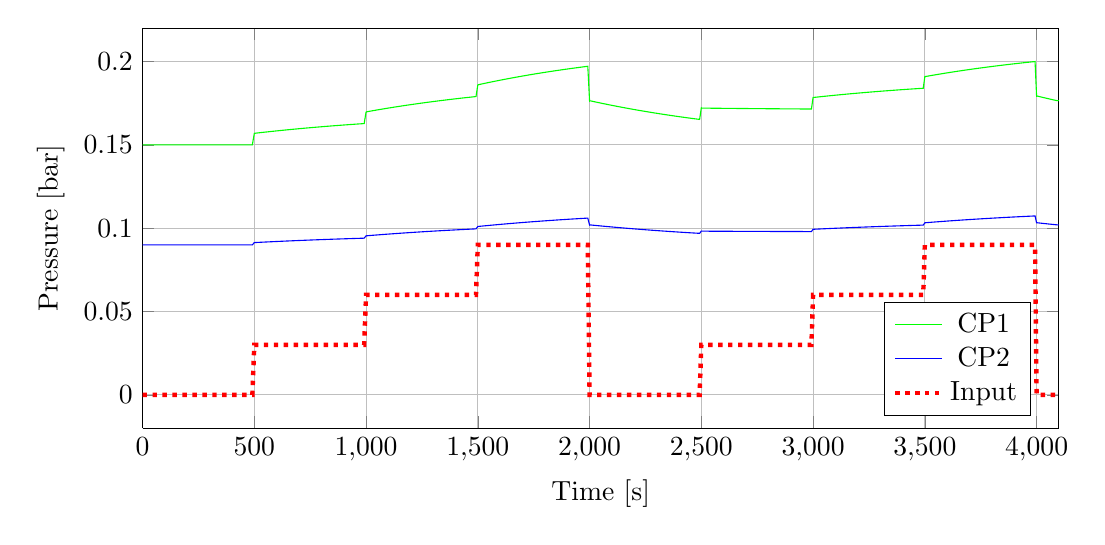
\begin{tikzpicture}

\begin{axis}[%
scaled y ticks = false,
 y tick label style={/pgf/number format/fixed,
/pgf/number format/1000 sep = \thinspace}, % Optional if you want to replace comma as the 1000 separator 
width=4.582in,
height=2in,
at={(0.303in,0.41in)},
scale only axis,
separate axis lines,
every outer x axis line/.append style={black},
every x tick label/.append style={font=\color{black}},
xmin=0,
xmax=4100,
xlabel={Time [s]},
xmajorgrids,
every outer y axis line/.append style={black},
every y tick label/.append style={font=\color{black}},
ymin=-0.02,
ymax=0.22,
ymajorgrids,
ylabel={Pressure [bar]},
legend pos=south east,
axis background/.style={fill=white}
]
\addplot [color=green,solid]
  table[row sep=crcr]{
0	0.15\\
8.93323388268949	0.15\\
17.866467765379	0.15\\
26.7997016480685	0.15\\
35.732935530758	0.15\\
44.6661694134474	0.15\\
53.5994032961369	0.15\\
62.5326371788264	0.15\\
71.4658710615159	0.15\\
80.3991049442054	0.15\\
89.3323388268949	0.15\\
98.2655727095844	0.15\\
107.198806592274	0.15\\
116.132040474963	0.15\\
125.065274357653	0.15\\
133.998508240342	0.15\\
142.931742123032	0.15\\
151.864976005721	0.15\\
160.798209888411	0.15\\
169.7314437711	0.15\\
178.66467765379	0.15\\
187.597911536479	0.15\\
196.531145419169	0.15\\
205.464379301858	0.15\\
214.397613184548	0.15\\
223.330847067237	0.15\\
232.264080949927	0.15\\
241.197314832616	0.15\\
250.130548715306	0.15\\
259.063782597995	0.15\\
267.997016480685	0.15\\
276.930250363374	0.15\\
285.863484246064	0.15\\
294.796718128753	0.15\\
303.729952011443	0.15\\
312.663185894132	0.15\\
321.596419776822	0.15\\
330.529653659511	0.15\\
339.462887542201	0.15\\
348.39612142489	0.15\\
357.32935530758	0.15\\
366.262589190269	0.15\\
375.195823072959	0.15\\
384.129056955648	0.15\\
393.062290838338	0.15\\
401.995524721027	0.15\\
410.928758603717	0.15\\
419.861992486406	0.15\\
428.795226369095	0.15\\
437.728460251785	0.15\\
446.661694134474	0.15\\
455.594928017164	0.15\\
464.528161899853	0.15\\
473.461395782543	0.15\\
482.394629665232	0.15\\
491.327863547922	0.15\\
500	0.156936442437769\\
500.261097430611	0.156936442437769\\
509.194331313301	0.15707406453234\\
518.12756519599	0.157210317263982\\
527.06079907868	0.157345214258088\\
535.994032961369	0.157478769004471\\
544.927266844059	0.157610994858723\\
553.860500726748	0.157741905043543\\
562.793734609438	0.157871512650062\\
571.726968492127	0.157999830639154\\
580.660202374817	0.158126871842727\\
589.593436257506	0.158252648965012\\
598.526670140196	0.158377174583831\\
607.459904022885	0.158500461151851\\
616.393137905575	0.158622520997838\\
625.326371788264	0.15874336632788\\
634.259605670954	0.158863009226615\\
643.192839553643	0.158981461658436\\
652.126073436333	0.159098735468689\\
661.059307319022	0.159214842384857\\
669.992541201712	0.15932979401773\\
678.925775084401	0.159443601862572\\
687.859008967091	0.159556277300265\\
696.79224284978	0.159667831598451\\
705.72547673247	0.159778275912656\\
714.658710615159	0.159887621287406\\
723.591944497849	0.159995878657334\\
732.525178380538	0.160103058848269\\
741.458412263228	0.160209172578324\\
750.391646145917	0.160314230458964\\
759.324880028607	0.160418242996066\\
768.258113911296	0.160521220590976\\
777.191347793986	0.16062317354154\\
786.124581676675	0.160724112043143\\
795.057815559364	0.160824046189721\\
803.991049442054	0.160922985974776\\
812.924283324744	0.161020941292372\\
821.857517207433	0.161117921938124\\
830.790751090123	0.161213937610182\\
839.723984972812	0.161308997910195\\
848.657218855501	0.161403112344276\\
857.590452738191	0.161496290323949\\
866.52368662088	0.161588541167093\\
875.45692050357	0.161679874098871\\
884.390154386259	0.161770298252656\\
893.323388268949	0.161859822670942\\
902.256622151638	0.161948456306247\\
911.189856034328	0.162036208022011\\
920.123089917017	0.162123086593483\\
929.056323799707	0.162209100708593\\
937.989557682396	0.162294258968829\\
946.922791565086	0.162378569890088\\
955.856025447775	0.162462041903538\\
964.789259330465	0.16254468335645\\
973.722493213154	0.162626502513042\\
982.655727095844	0.1627075075553\\
991.588960978533	0.162787706583798\\
1000	0.169724149021567\\
1000.52219486122	0.169803550056277\\
1009.45542874391	0.170019783131943\\
1018.3886626266	0.17023386465223\\
1027.32189650929	0.170445816025477\\
1036.25513039198	0.170655658447002\\
1045.18836427467	0.170863412901231\\
1054.12159815736	0.171069100163787\\
1063.05483204005	0.171272740803574\\
1071.98806592274	0.171474355184833\\
1080.92129980543	0.171673963469175\\
1089.85453368812	0.171871585617602\\
1098.78776757081	0.172067241392499\\
1107.7210014535	0.172260950359612\\
1116.65423533619	0.172452731890007\\
1125.58746921888	0.172642605162\\
1134.52070310157	0.172830589163084\\
1143.45393698425	0.173016702691821\\
1152.38717086694	0.173200964359725\\
1161.32040474963	0.173383392593121\\
1170.25363863232	0.173564005634991\\
1179.18687251501	0.173742821546794\\
1188.1201063977	0.173919858210277\\
1197.05334028039	0.174095133329259\\
1205.98657416308	0.174268664431403\\
1214.91980804577	0.174440468869969\\
1223.85304192846	0.174610563825549\\
1232.78627581115	0.174778966307786\\
1241.71950969384	0.174945693157073\\
1250.65274357653	0.17511076104624\\
1259.58597745922	0.175274186482218\\
1268.51921134191	0.175435985807692\\
1277.4524452246	0.175596175202734\\
1286.38567910729	0.175754770686422\\
1295.31891298998	0.175911788118441\\
1304.25214687267	0.17606724320067\\
1313.18538075535	0.176221151478752\\
1322.11861463804	0.176373528343648\\
1331.05184852073	0.176524389033175\\
1339.98508240342	0.176673748633532\\
1348.91831628611	0.17682162208081\\
1357.8515501688	0.17696802416248\\
1366.78478405149	0.177112969518877\\
1375.71801793418	0.177256472644662\\
1384.65125181687	0.177398547890271\\
1393.58448569956	0.177539209463352\\
1402.51771958225	0.177678471430183\\
1411.45095346494	0.177816347717082\\
1420.38418734763	0.177952852111796\\
1429.31742123032	0.178087998264883\\
1438.25065511301	0.178221799691074\\
1447.1838889957	0.178354269770628\\
1456.11712287839	0.178485421750667\\
1465.05035676108	0.178615268746503\\
1473.98359064377	0.178743823742948\\
1482.91682452646	0.178871099595611\\
1491.85005840914	0.178997109032188\\
1500	0.185933551469957\\
1500.78329229183	0.186058307091501\\
1509.71652617452	0.186319443468253\\
1518.64976005721	0.186577981494248\\
1527.5829939399	0.186833947023512\\
1536.51622782259	0.187087365652819\\
1545.44946170528	0.187338262724251\\
1554.38269558797	0.187586663327732\\
1563.31592947066	0.187832592303537\\
1572.24916335335	0.188076074244775\\
1581.18239723604	0.188317133499851\\
1590.11563111873	0.1885557941749\\
1599.04886500142	0.188792080136193\\
1607.98209888411	0.189026015012533\\
1616.9153327668	0.189257622197608\\
1625.84856664949	0.189486924852337\\
1634.78180053218	0.189713945907184\\
1643.71503441487	0.18993870806445\\
1652.64826829756	0.190161233800545\\
1661.58150218025	0.190381545368235\\
1670.51473606293	0.190599664798868\\
1679.44796994562	0.190815613904573\\
1688.38120382831	0.191029414280449\\
1697.314437711	0.191241087306719\\
1706.24767159369	0.191450654150866\\
1715.18090547638	0.191658135769757\\
1724.11413935907	0.191863552911734\\
1733.04737324176	0.192066926118686\\
1741.98060712445	0.192268275728112\\
1750.91384100714	0.192467621875146\\
1759.84707488983	0.192664984494574\\
1768.78030877252	0.192860383322829\\
1777.71354265521	0.193053837899963\\
1786.6467765379	0.193245367571601\\
1795.58001042059	0.193434991490875\\
1804.51324430328	0.193622728620341\\
1813.44647818597	0.193808597733874\\
1822.37971206866	0.193992617418545\\
1831.31294595135	0.194174806076484\\
1840.24617983403	0.194355181926711\\
1849.17941371672	0.194533763006969\\
1858.11264759941	0.19471056717552\\
1867.0458814821	0.194885612112933\\
1875.97911536479	0.195058915323853\\
1884.91234924748	0.195230494138752\\
1893.84558313017	0.195400365715658\\
1902.77881701286	0.195568547041876\\
1911.71205089555	0.195735054935684\\
1920.64528477824	0.195899906048015\\
1929.57851866093	0.196063116864124\\
1938.51175254362	0.196224703705231\\
1947.44498642631	0.196384682730162\\
1956.378220309	0.196543069936957\\
1965.31145419169	0.196699881164473\\
1974.24468807438	0.196855132093969\\
1983.17792195707	0.197008838250671\\
1992.11115583976	0.197161015005328\\
2000	0.176351687692023\\
2001.04438972245	0.176502350262442\\
2009.97762360514	0.176238647431297\\
2018.91085748782	0.175977568487561\\
2027.84409137051	0.175719087323113\\
2036.7773252532	0.175463178089615\\
2045.71055913589	0.175209815195921\\
2054.64379301858	0.174958973305523\\
2063.57702690127	0.174710627334017\\
2072.51026078396	0.174464752446589\\
2081.44349466665	0.174221324055539\\
2090.37672854934	0.173980317817817\\
2099.30996243203	0.173741709632593\\
2108.24319631472	0.17350547563884\\
2117.17643019741	0.173271592212955\\
2126.1096640801	0.173040035966394\\
2135.04289796279	0.172810783743333\\
2143.97613184548	0.17258381261835\\
2152.90936572817	0.172359099894138\\
2161.84259961086	0.172136623099229\\
2170.77583349355	0.171916359985752\\
2179.70906737624	0.171698288527206\\
2188.64230125892	0.171482386916256\\
2197.57553514161	0.171268633562554\\
2206.5087690243	0.171057007090581\\
2215.44200290699	0.170847486337507\\
2224.37523678968	0.170640050351075\\
2233.30847067237	0.170434678387507\\
2242.24170455506	0.17023134990943\\
2251.17493843775	0.170030044583821\\
2260.10817232044	0.169830742279972\\
2269.04140620313	0.169633423067481\\
2277.97464008582	0.169438067214257\\
2286.90787396851	0.169244655184546\\
2295.8411078512	0.169053167636976\\
2304.77434173389	0.16886358542263\\
2313.70757561658	0.16867588958312\\
2322.64080949927	0.168490061348701\\
2331.57404338196	0.168306082136389\\
2340.50727726465	0.168123933548104\\
2349.44051114734	0.16794359736883\\
2358.37374503003	0.167765055564792\\
2367.30697891271	0.167588290281657\\
2376.2402127954	0.167413283842744\\
2385.17344667809	0.167240018747256\\
2394.10668056078	0.167068477668536\\
2403.03991444347	0.166898643452326\\
2411.97314832616	0.16673049911506\\
2420.90638220885	0.166564027842157\\
2429.83961609154	0.166399212986346\\
2438.77284997423	0.166236038066\\
2447.70608385692	0.166074486763486\\
2456.63931773961	0.165914542923534\\
2465.5725516223	0.165756190551622\\
2474.50578550499	0.165599413812375\\
2483.43901938768	0.165444197027984\\
2492.37225327037	0.165290524676638\\
2500	0.172226967114406\\
2501.30548715306	0.172074823828736\\
2510.23872103575	0.172061816488852\\
2519.17195491844	0.172048938574183\\
2528.10518880113	0.172036188796925\\
2537.03842268382	0.172023565882089\\
2545.9716565665	0.172011068567374\\
2554.90489044919	0.171998695603036\\
2563.83812433188	0.17198644575177\\
2572.77135821457	0.171974317788579\\
2581.70459209726	0.171962310500656\\
2590.63782597995	0.171950422687262\\
2599.57105986264	0.171938653159605\\
2608.50429374533	0.171927000740724\\
2617.43752762802	0.171915464265365\\
2626.37076151071	0.171904042579871\\
2635.3039953934	0.171892734542064\\
2644.23722927609	0.17188153902113\\
2653.17046315878	0.171870454897508\\
2662.10369704147	0.171859481062775\\
2671.03693092416	0.171848616419539\\
2679.97016480685	0.171837859881325\\
2688.90339868954	0.171827210372472\\
2697.83663257223	0.171816666828018\\
2706.76986645492	0.1718062281936\\
2715.7031003376	0.171795893425346\\
2724.63633422029	0.171785661489769\\
2733.56956810298	0.171775531363668\\
2742.50280198567	0.171765502034022\\
2751.43603586836	0.171755572497887\\
2760.36926975105	0.171745741762303\\
2769.30250363374	0.171736008844188\\
2778.23573751643	0.17172637277024\\
2787.16897139912	0.171716832576845\\
2796.10220528181	0.171707387309974\\
2805.0354391645	0.171698036025094\\
2813.96867304719	0.171688777787066\\
2822.90190692988	0.17167961167006\\
2831.83514081257	0.171670536757457\\
2840.76837469526	0.171661552141756\\
2849.70160857795	0.171652656924488\\
2858.63484246064	0.171643850216124\\
2867.56807634333	0.171635131135987\\
2876.50131022602	0.171626498812159\\
2885.4345441087	0.171617952381401\\
2894.36777799139	0.171609490989064\\
2903.30101187408	0.171601113788999\\
2912.23424575677	0.171592819943481\\
2921.16747963946	0.171584608623116\\
2930.10071352215	0.171576479006767\\
2939.03394740484	0.171568430281465\\
2947.96718128753	0.171560461642329\\
2956.90041517022	0.17155257229249\\
2965.83364905291	0.171544761443005\\
2974.7668829356	0.171537028312783\\
2983.70011681829	0.171529372128504\\
2992.63335070098	0.171521792124542\\
3000	0.178458234562311\\
3001.56658458367	0.178450729980661\\
3010.49981846636	0.178580922165428\\
3019.43305234905	0.178709818916116\\
3028.36628623174	0.178837433122511\\
3037.29952011443	0.178963777546144\\
3046.23275399712	0.179088864821566\\
3055.16598787981	0.179212707457613\\
3064.09922176249	0.179335317838655\\
3073.03245564518	0.179456708225837\\
3081.96568952787	0.179576890758302\\
3090.89892341056	0.179695877454407\\
3099.83215729325	0.179813680212925\\
3108.76539117594	0.179930310814233\\
3117.69862505863	0.180045780921492\\
3126.63185894132	0.180160102081812\\
3135.56509282401	0.180273285727409\\
3144.4983267067	0.180385343176744\\
3153.43156058939	0.18049628563566\\
3162.36479447208	0.180606124198498\\
3171.29802835477	0.180714869849209\\
3180.23126223746	0.180822533462452\\
3189.16449612015	0.180929125804682\\
3198.09773000284	0.181034657535225\\
3207.03096388553	0.181139139207345\\
3215.96419776822	0.181242581269299\\
3224.89743165091	0.181344994065384\\
3233.8306655336	0.181446387836966\\
3242.76389941628	0.181546772723512\\
3251.69713329897	0.181646158763596\\
3260.63036718166	0.181744555895908\\
3269.56360106435	0.181841973960247\\
3278.49683494704	0.181938422698502\\
3287.43006882973	0.182033911755632\\
3296.36330271242	0.182128450680624\\
3305.29653659511	0.182222048927452\\
3314.2297704778	0.182314715856023\\
3323.16300436049	0.182406460733108\\
3332.09623824318	0.182497292733275\\
3341.02947212587	0.182587220939803\\
3349.96270600856	0.182676254345589\\
3358.89593989125	0.182764401854052\\
3367.82917377394	0.182851672280017\\
3376.76240765663	0.182938074350604\\
3385.69564153932	0.183023616706094\\
3394.62887542201	0.183108307900796\\
3403.5621093047	0.183192156403903\\
3412.49534318738	0.183275170600337\\
3421.42857707007	0.183357358791591\\
3430.36181095276	0.183438729196554\\
3439.29504483545	0.183519289952336\\
3448.22827871814	0.183599049115084\\
3457.16151260083	0.183678014660782\\
3466.09474648352	0.183756194486053\\
3475.02798036621	0.183833596408947\\
3483.9612142489	0.183910228169724\\
3492.89444813159	0.183986097431625\\
3500	0.190922539869393\\
3501.82768201428	0.19099765421941\\
3510.76091589697	0.191209643263615\\
3519.69414977966	0.191419522981266\\
3528.62738366235	0.191627314360518\\
3537.56061754504	0.191833038180686\\
3546.49385142773	0.192036715014332\\
3555.42708531042	0.192238365229315\\
3564.36031919311	0.192438008990829\\
3573.2935530758	0.192635666263424\\
3582.22678695849	0.192831356812998\\
3591.16002084117	0.193025100208774\\
3600.09325472386	0.19321691582526\\
3609.02648860655	0.193406822844183\\
3617.95972248924	0.193594840256409\\
3626.89295637193	0.193780986863842\\
3635.82619025462	0.193965281281302\\
3644.75942413731	0.194147741938392\\
3653.69265802	0.194328387081334\\
3662.62589190269	0.194507234774799\\
3671.55912578538	0.19468430290371\\
3680.49235966807	0.194859609175034\\
3689.42559355076	0.195033171119548\\
3698.35882743345	0.195205006093598\\
3707.29206131614	0.195375131280829\\
3716.22529519883	0.195543563693907\\
3725.15852908152	0.195710320176219\\
3734.09176296421	0.195875417403556\\
3743.0249968469	0.196038871885785\\
3751.95823072959	0.196200699968495\\
3760.89146461227	0.196360917834633\\
3769.82469849496	0.196519541506125\\
3778.75793237765	0.196676586845475\\
3787.69116626034	0.196832069557353\\
3796.62440014303	0.196986005190163\\
3805.55763402572	0.197138409137603\\
3814.49086790841	0.197289296640199\\
3823.4241017911	0.197438682786831\\
3832.35733567379	0.197586582516243\\
3841.29056955648	0.197733010618535\\
3850.22380343917	0.197877981736645\\
3859.15703732186	0.19802151036781\\
3868.09027120455	0.198163610865016\\
3877.02350508724	0.198304297438436\\
3885.95673896993	0.198443584156849\\
3894.88997285262	0.198581484949047\\
3903.82320673531	0.198718013605228\\
3912.756440618	0.198853183778376\\
3921.68967450069	0.198987008985626\\
3930.62290838338	0.199119502609612\\
3939.55614226606	0.199250677899813\\
3948.48937614875	0.199380547973871\\
3957.42261003144	0.199509125818904\\
3966.35584391413	0.19963642429281\\
3975.28907779682	0.199762456125544\\
3984.22231167951	0.199887233920399\\
3993.1555455622	0.200010770155263\\
4000	0.179201442841958\\
4002.08877944489	0.17932374987056\\
4011.02201332758	0.179031973639997\\
4019.95524721027	0.178743100631875\\
4028.88848109296	0.178457101958646\\
4037.82171497565	0.178173949020195\\
4046.75494885834	0.177893613500983\\
4055.68818274103	0.177616067367216\\
4064.62141662372	0.177341282864042\\
4073.55465050641	0.177069232512771\\
4082.4878843891	0.176799889108135\\
4091.42111827179	0.176533225715561\\
4100	0.176533225715561\\
};
\addlegendentry{CP1};

\addplot [color=blue,solid]
  table[row sep=crcr]{
0	0.09\\
8.93323388268949	0.09\\
17.866467765379	0.09\\
26.7997016480685	0.09\\
35.732935530758	0.09\\
44.6661694134474	0.09\\
53.5994032961369	0.09\\
62.5326371788264	0.09\\
71.4658710615159	0.09\\
80.3991049442054	0.09\\
89.3323388268949	0.09\\
98.2655727095844	0.09\\
107.198806592274	0.09\\
116.132040474963	0.09\\
125.065274357653	0.09\\
133.998508240342	0.09\\
142.931742123032	0.09\\
151.864976005721	0.09\\
160.798209888411	0.09\\
169.7314437711	0.09\\
178.66467765379	0.09\\
187.597911536479	0.09\\
196.531145419169	0.09\\
205.464379301858	0.09\\
214.397613184548	0.09\\
223.330847067237	0.09\\
232.264080949927	0.09\\
241.197314832616	0.09\\
250.130548715306	0.09\\
259.063782597995	0.09\\
267.997016480685	0.09\\
276.930250363374	0.09\\
285.863484246064	0.09\\
294.796718128753	0.09\\
303.729952011443	0.09\\
312.663185894132	0.09\\
321.596419776822	0.09\\
330.529653659511	0.09\\
339.462887542201	0.09\\
348.39612142489	0.09\\
357.32935530758	0.09\\
366.262589190269	0.09\\
375.195823072959	0.09\\
384.129056955648	0.09\\
393.062290838338	0.09\\
401.995524721027	0.09\\
410.928758603717	0.09\\
419.861992486406	0.09\\
428.795226369095	0.09\\
437.728460251785	0.09\\
446.661694134474	0.09\\
455.594928017164	0.09\\
464.528161899853	0.09\\
473.461395782543	0.09\\
482.394629665232	0.09\\
491.327863547922	0.09\\
500	0.0913793606916084\\
500.261097430611	0.0913793606916084\\
509.194331313301	0.0914417192209037\\
518.12756519599	0.0915034572723712\\
527.06079907868	0.0915645810198695\\
535.994032961369	0.091625096575826\\
544.927266844059	0.0916850099918487\\
553.860500726748	0.0917443272593309\\
562.793734609438	0.0918030543100506\\
571.726968492127	0.0918611970167635\\
580.660202374817	0.0919187611937907\\
589.593436257506	0.0919757525975994\\
598.526670140196	0.0920321769273794\\
607.459904022885	0.0920880398256124\\
616.393137905575	0.0921433468786363\\
625.326371788264	0.0921981036172044\\
634.259605670954	0.0922523155170377\\
643.192839553643	0.0923059879993731\\
652.126073436333	0.0923591264315052\\
661.059307319022	0.092411736127323\\
669.992541201712	0.0924638223478416\\
678.925775084401	0.0925153903017282\\
687.859008967091	0.0925664451458225\\
696.79224284978	0.0926169919856531\\
705.72547673247	0.0926670358759476\\
714.658710615159	0.0927165818211384\\
723.591944497849	0.0927656347758627\\
732.525178380538	0.0928141996454583\\
741.458412263228	0.0928622812864543\\
750.391646145917	0.0929098845070561\\
759.324880028607	0.092957014067627\\
768.258113911296	0.0930036746811639\\
777.191347793986	0.0930498710137682\\
786.124581676675	0.0930956076851132\\
795.057815559364	0.0931408892689056\\
803.991049442054	0.0931857202933428\\
812.924283324744	0.093230105241566\\
821.857517207433	0.0932740485521083\\
830.790751090123	0.0933175546193389\\
839.723984972812	0.0933606277939019\\
848.657218855501	0.093403272383152\\
857.590452738191	0.0934454926515851\\
866.52368662088	0.0934872928212643\\
875.45692050357	0.0935286770722429\\
884.390154386259	0.0935696495429816\\
893.323388268949	0.0936102143307629\\
902.256622151638	0.0936503754921007\\
911.189856034328	0.0936901370431457\\
920.123089917017	0.0937295029600874\\
929.056323799707	0.0937684771795515\\
937.989557682396	0.0938070635989936\\
946.922791565086	0.0938452660770891\\
955.856025447775	0.0938830884341186\\
964.789259330465	0.0939205344523506\\
973.722493213154	0.0939576078764193\\
982.655727095844	0.093994312413699\\
991.588960978533	0.0940306517346752\\
1000	0.0954100124262836\\
1000.52219486122	0.0954459901649199\\
1009.45542874391	0.0955439684483164\\
1018.3886626266	0.0956409718313562\\
1027.32189650929	0.0957370100144616\\
1036.25513039198	0.0958320926015336\\
1045.18836427467	0.0959262291009133\\
1054.12159815736	0.0960194289263318\\
1063.05483204005	0.0961117013978521\\
1071.98806592274	0.0962030557428012\\
1080.92129980543	0.0962935010966925\\
1089.85453368812	0.0963830465041395\\
1098.78776757081	0.0964717009197602\\
1107.7210014535	0.0965594732090728\\
1116.65423533619	0.096646372149382\\
1125.58746921888	0.0967324064306571\\
1134.52070310157	0.0968175846564003\\
1143.45393698425	0.0969019153445079\\
1152.38717086694	0.0969854069281215\\
1161.32040474963	0.0970680677564717\\
1170.25363863232	0.0971499060957125\\
1179.18687251501	0.0972309301297487\\
1188.1201063977	0.0973111479610537\\
1197.05334028039	0.0973905676114798\\
1205.98657416308	0.0974691970230607\\
1214.91980804577	0.0975470440588056\\
1223.85304192846	0.0976241165034852\\
1232.78627581115	0.0977004220644105\\
1241.71950969384	0.0977759683722036\\
1250.65274357653	0.0978507629815605\\
1259.58597745922	0.0979248133720068\\
1268.51921134191	0.0979981269486455\\
1277.4524452246	0.0980707110428975\\
1286.38567910729	0.098142572913235\\
1295.31891298998	0.0982137197459071\\
1304.25214687267	0.0982841586556585\\
1313.18538075535	0.0983538966864411\\
1322.11861463804	0.0984229408121181\\
1331.05184852073	0.0984912979371618\\
1339.98508240342	0.0985589748973437\\
1348.91831628611	0.0986259784604183\\
1357.8515501688	0.0986923153267998\\
1366.78478405149	0.0987579921302322\\
1375.71801793418	0.0988230154384524\\
1384.65125181687	0.0988873917538476\\
1393.58448569956	0.0989511275141048\\
1402.51771958225	0.0990142290928551\\
1411.45095346494	0.099076702800311\\
1420.38418734763	0.0991385548838971\\
1429.31742123032	0.0991997915288751\\
1438.25065511301	0.0992604188589627\\
1447.1838889957	0.0993204429369449\\
1456.11712287839	0.0993798697652817\\
1465.05035676108	0.099438705286707\\
1473.98359064377	0.0994969553848239\\
1482.91682452646	0.0995546258846925\\
1491.85005840914	0.0996117225534126\\
1500	0.100991083245021\\
1500.78329229183	0.101047611792309\\
1509.71652617452	0.101165936400363\\
1518.64976005721	0.101283083658717\\
1527.5829939399	0.101399065282198\\
1536.51622782259	0.101513892869068\\
1545.44946170528	0.101627577902186\\
1554.38269558797	0.101740131750152\\
1563.31592947066	0.101851565668448\\
1572.24916335335	0.101961890800564\\
1581.18239723604	0.102071118179107\\
1590.11563111873	0.102179258726909\\
1599.04886500142	0.102286323258119\\
1607.98209888411	0.102392322479282\\
1616.9153327668	0.102497266990413\\
1625.84856664949	0.102601167286052\\
1634.78180053218	0.102704033756319\\
1643.71503441487	0.10280587668795\\
1652.64826829756	0.102906706265326\\
1661.58150218025	0.103006532571493\\
1670.51473606293	0.103105365589166\\
1679.44796994562	0.103203215201732\\
1688.38120382831	0.103300091194239\\
1697.314437711	0.103396003254368\\
1706.24767159369	0.103490960973409\\
1715.18090547638	0.103584973847215\\
1724.11413935907	0.103678051277156\\
1733.04737324176	0.103770202571053\\
1741.98060712445	0.103861436944117\\
1750.91384100714	0.103951763519864\\
1759.84707488983	0.104041191331029\\
1768.78030877252	0.10412972932047\\
1777.71354265521	0.104217386342063\\
1786.6467765379	0.104304171161586\\
1795.58001042059	0.104390092457596\\
1804.51324430328	0.104475158822296\\
1813.44647818597	0.104559378762397\\
1822.37971206866	0.104642760699965\\
1831.31294595135	0.104725312973266\\
1840.24617983403	0.104807043837599\\
1849.17941371672	0.10488796146612\\
1858.11264759941	0.104968073950663\\
1867.0458814821	0.105047389302545\\
1875.97911536479	0.10512591545337\\
1884.91234924748	0.105203660255821\\
1893.84558313017	0.105280631484445\\
1902.77881701286	0.105356836836431\\
1911.71205089555	0.105432283932381\\
1920.64528477824	0.105506980317069\\
1929.57851866093	0.105580933460199\\
1938.51175254362	0.105654150757148\\
1947.44498642631	0.105726639529709\\
1956.378220309	0.105798407026823\\
1965.31145419169	0.1058694604253\\
1974.24468807438	0.105939806830543\\
1983.17792195707	0.106009453277252\\
1992.11115583976	0.106078406730133\\
2000	0.101940324655308\\
2001.04438972245	0.102008592009765\\
2009.97762360514	0.101889104504707\\
2018.91085748782	0.101770805920369\\
2027.84409137051	0.101653684426791\\
2036.7773252532	0.101537728311723\\
2045.71055913589	0.101422925979452\\
2054.64379301858	0.101309265949647\\
2063.57702690127	0.101196736856206\\
2072.51026078396	0.101085327446122\\
2081.44349466665	0.100975026578359\\
2090.37672854934	0.100865823222734\\
2099.30996243203	0.100757706458817\\
2108.24319631472	0.10065066547484\\
2117.17643019741	0.100544689566609\\
2126.1096640801	0.100439768136445\\
2135.04289796279	0.100335890692112\\
2143.97613184548	0.100233046845777\\
2152.90936572817	0.100131226312965\\
2161.84259961086	0.100030418911537\\
2170.77583349355	0.0999306145606644\\
2179.70906737624	0.0998318032798261\\
2188.64230125892	0.0997339751878088\\
2197.57553514161	0.0996371205017186\\
2206.5087690243	0.0995412295360034\\
2215.44200290699	0.0994462927014837\\
2224.37523678968	0.0993523005043941\\
2233.30847067237	0.0992592435454336\\
2242.24170455506	0.0991671125188261\\
2251.17493843775	0.0990758982113891\\
2260.10817232044	0.0989855915016133\\
2269.04140620313	0.0988961833587496\\
2277.97464008582	0.0988076648419066\\
2286.90787396851	0.0987200270991559\\
2295.8411078512	0.0986332613666478\\
2304.77434173389	0.0985473589677339\\
2313.70757561658	0.0984623113121002\\
2322.64080949927	0.0983781098949076\\
2331.57404338196	0.0982947462959418\\
2340.50727726465	0.0982122121787707\\
2349.44051114734	0.0981304992899114\\
2358.37374503003	0.0980495994580044\\
2367.30697891271	0.0979695045929966\\
2376.2402127954	0.0978902066853324\\
2385.17344667809	0.0978116978051524\\
2394.10668056078	0.0977339701015009\\
2403.03991444347	0.0976570158015403\\
2411.97314832616	0.0975808272097742\\
2420.90638220885	0.0975053967072775\\
2429.83961609154	0.0974307167509349\\
2438.77284997423	0.0973567798726862\\
2447.70608385692	0.0972835786787798\\
2456.63931773961	0.0972111058490329\\
2465.5725516223	0.0971393541361001\\
2474.50578550499	0.097068316364748\\
2483.43901938768	0.0969979854311381\\
2492.37225327037	0.0969283543021164\\
2500	0.0983077149937248\\
2501.30548715306	0.0982387767061182\\
2510.23872103575	0.0982328828953336\\
2519.17195491844	0.0982270477289551\\
2528.10518880113	0.098221270623461\\
2537.03842268382	0.0982155510011357\\
2545.9716565665	0.098209888290012\\
2554.90489044919	0.0982042819238141\\
2563.83812433188	0.0981987313419003\\
2572.77135821457	0.0981932359892077\\
2581.70459209726	0.0981877953161963\\
2590.63782597995	0.0981824087787941\\
2599.57105986264	0.0981770758383427\\
2608.50429374533	0.0981717959615434\\
2617.43752762802	0.0981665686204041\\
2626.37076151071	0.098161393292186\\
2635.3039953934	0.0981562694593519\\
2644.23722927609	0.0981511966095141\\
2653.17046315878	0.0981461742353832\\
2662.10369704147	0.0981412018347174\\
2671.03693092416	0.0981362789102725\\
2679.97016480685	0.0981314049697516\\
2688.90339868954	0.0981265795257566\\
2697.83663257223	0.0981218020957388\\
2706.76986645492	0.0981170722019512\\
2715.7031003376	0.0981123893714002\\
2724.63633422029	0.0981077531357989\\
2733.56956810298	0.0981031630315195\\
2742.50280198567	0.0980986185995477\\
2751.43603586836	0.0980941193854365\\
2760.36926975105	0.0980896649392604\\
2769.30250363374	0.0980852548155711\\
2778.23573751643	0.0980808885733523\\
2787.16897139912	0.0980765657759761\\
2796.10220528181	0.0980722859911589\\
2805.0354391645	0.0980680487909187\\
2813.96867304719	0.0980638537515317\\
2822.90190692988	0.0980597004534903\\
2831.83514081257	0.0980555884814612\\
2840.76837469526	0.0980515174242437\\
2849.70160857795	0.0980474868747284\\
2858.63484246064	0.0980434964298569\\
2867.56807634333	0.0980395456905814\\
2876.50131022602	0.0980356342618244\\
2885.4345441087	0.0980317617524397\\
2894.36777799139	0.0980279277751731\\
2903.30101187408	0.0980241319466235\\
2912.23424575677	0.0980203738872047\\
2921.16747963946	0.0980166532211076\\
2930.10071352215	0.0980129695762623\\
2939.03394740484	0.0980093225843012\\
2947.96718128753	0.0980057118805219\\
2956.90041517022	0.098002137103851\\
2965.83364905291	0.0979985978968077\\
2974.7668829356	0.0979950939054681\\
2983.70011681829	0.0979916247794303\\
2992.63335070098	0.0979881901717785\\
3000	0.0993675508633868\\
3001.56658458367	0.0993641504306573\\
3010.49981846636	0.0994231423620993\\
3019.43305234905	0.0994815473139269\\
3028.36628623174	0.0995393711266857\\
3037.29952011443	0.0995966195828072\\
3046.23275399712	0.0996532984071862\\
3055.16598787981	0.0997094132677542\\
3064.09922176249	0.0997649697760457\\
3073.03245564518	0.0998199734877596\\
3081.96568952787	0.0998744299033145\\
3090.89892341056	0.099928344468399\\
3099.83215729325	0.0999817225745162\\
3108.76539117594	0.100034569559523\\
3117.69862505863	0.100086890708163\\
3126.63185894132	0.100138691252597\\
3135.56509282401	0.100189976372924\\
3144.4983267067	0.100240751197699\\
3153.43156058939	0.100291020804451\\
3162.36479447208	0.100340790220182\\
3171.29802835477	0.100390064421877\\
3180.23126223746	0.100438848336999\\
3189.16449612015	0.100487146843981\\
3198.09773000284	0.100534964772717\\
3207.03096388553	0.100582306905039\\
3215.96419776822	0.100629177975203\\
3224.89743165091	0.100675582670356\\
3233.8306655336	0.100721525631007\\
3242.76389941628	0.100767011451492\\
3251.69713329897	0.100812044680433\\
3260.63036718166	0.100856629821191\\
3269.56360106435	0.100900771332319\\
3278.49683494704	0.100944473628006\\
3287.43006882973	0.100987741078519\\
3296.36330271242	0.101030578010641\\
3305.29653659511	0.101072988708102\\
3314.2297704778	0.101114977412009\\
3323.16300436049	0.101156548321268\\
3332.09623824318	0.101197705593006\\
3341.02947212587	0.101238453342985\\
3349.96270600856	0.101278795646016\\
3358.89593989125	0.101318736536364\\
3367.82917377394	0.101358280008153\\
3376.76240765663	0.101397430015764\\
3385.69564153932	0.101436190474231\\
3394.62887542201	0.101474565259634\\
3403.5621093047	0.101512558209485\\
3412.49534318738	0.10155017312311\\
3421.42857707007	0.101587413762035\\
3430.36181095276	0.101624283850355\\
3439.29504483545	0.101660787075111\\
3448.22827871814	0.101696927086657\\
3457.16151260083	0.101732707499025\\
3466.09474648352	0.101768131890288\\
3475.02798036621	0.101803203802915\\
3483.9612142489	0.101837926744127\\
3492.89444813159	0.101872304186249\\
3500	0.103251664877858\\
3501.82768201428	0.103285700258664\\
3510.76091589697	0.103381755511016\\
3519.69414977966	0.103476854997493\\
3528.62738366235	0.103571008228126\\
3537.56061754504	0.103664224618319\\
3546.49385142773	0.103756513489792\\
3555.42708531042	0.103847884071511\\
3564.36031919311	0.103938345500614\\
3573.2935530758	0.104027906823321\\
3582.22678695849	0.104116576995843\\
3591.16002084117	0.104204364885272\\
3600.09325472386	0.104291279270475\\
3609.02648860655	0.104377328842964\\
3617.95972248924	0.104462522207771\\
3626.89295637193	0.104546867884306\\
3635.82619025462	0.10463037430721\\
3644.75942413731	0.104713049827197\\
3653.69265802	0.104794902711891\\
3662.62589190269	0.10487594114665\\
3671.55912578538	0.104956173235388\\
3680.49235966807	0.105035607001383\\
3689.42559355076	0.105114250388082\\
3698.35882743345	0.105192111259889\\
3707.29206131614	0.10526919740296\\
3716.22529519883	0.105345516525975\\
3725.15852908152	0.105421076260913\\
3734.09176296421	0.105495884163812\\
3743.0249968469	0.105569947715528\\
3751.95823072959	0.105643274322479\\
3760.89146461227	0.10571587131739\\
3769.82469849496	0.105787745960023\\
3778.75793237765	0.105858905437904\\
3787.69116626034	0.105929356867042\\
3796.62440014303	0.105999107292641\\
3805.55763402572	0.106068163689805\\
3814.49086790841	0.106136532964231\\
3823.4241017911	0.106204221952908\\
3832.35733567379	0.106271237424791\\
3841.29056955648	0.106337586081487\\
3850.22380343917	0.106403274557918\\
3859.15703732186	0.106468309422989\\
3868.09027120455	0.106532697180242\\
3877.02350508724	0.106596444268509\\
3885.95673896993	0.106659557062553\\
3894.88997285262	0.106722041873708\\
3903.82320673531	0.106783904950511\\
3912.756440618	0.10684515247932\\
3921.68967450069	0.106905790584944\\
3930.62290838338	0.106965825331243\\
3939.55614226606	0.107025262721746\\
3948.48937614875	0.107084108700242\\
3957.42261003144	0.10714236915138\\
3966.35584391413	0.107200049901255\\
3975.28907779682	0.107257156717992\\
3984.22231167951	0.107313695312323\\
3993.1555455622	0.107369671338155\\
4000	0.10323158926333\\
4002.08877944489	0.103287008318315\\
4011.02201332758	0.103154800356519\\
4019.95524721027	0.103023907886123\\
4028.88848109296	0.102894317817766\\
4037.82171497565	0.102766017192328\\
4046.75494885834	0.102638993179638\\
4055.68818274103	0.102513233077183\\
4064.62141662372	0.102388724308846\\
4073.55465050641	0.10226545442364\\
4082.4878843891	0.102143411094473\\
4091.42111827179	0.102022582116904\\
4100	0.102022582116904\\
};
\addlegendentry{CP2};

\addplot [color=red,dotted,ultra thick]
  table[row sep=crcr]{
0	0\\
8.93323388268949	0\\
17.866467765379	0\\
26.7997016480685	0\\
35.732935530758	0\\
44.6661694134474	0\\
53.5994032961369	0\\
62.5326371788264	0\\
71.4658710615159	0\\
80.3991049442054	0\\
89.3323388268949	0\\
98.2655727095844	0\\
107.198806592274	0\\
116.132040474963	0\\
125.065274357653	0\\
133.998508240342	0\\
142.931742123032	0\\
151.864976005721	0\\
160.798209888411	0\\
169.7314437711	0\\
178.66467765379	0\\
187.597911536479	0\\
196.531145419169	0\\
205.464379301858	0\\
214.397613184548	0\\
223.330847067237	0\\
232.264080949927	0\\
241.197314832616	0\\
250.130548715306	0\\
259.063782597995	0\\
267.997016480685	0\\
276.930250363374	0\\
285.863484246064	0\\
294.796718128753	0\\
303.729952011443	0\\
312.663185894132	0\\
321.596419776822	0\\
330.529653659511	0\\
339.462887542201	0\\
348.39612142489	0\\
357.32935530758	0\\
366.262589190269	0\\
375.195823072959	0\\
384.129056955648	0\\
393.062290838338	0\\
401.995524721027	0\\
410.928758603717	0\\
419.861992486406	0\\
428.795226369095	0\\
437.728460251785	0\\
446.661694134474	0\\
455.594928017164	0\\
464.528161899853	0\\
473.461395782543	0\\
482.394629665232	0\\
491.327863547922	0\\
500	0.03\\
500.261097430611	0.03\\
509.194331313301	0.03\\
518.12756519599	0.03\\
527.06079907868	0.03\\
535.994032961369	0.03\\
544.927266844059	0.03\\
553.860500726748	0.03\\
562.793734609438	0.03\\
571.726968492127	0.03\\
580.660202374817	0.03\\
589.593436257506	0.03\\
598.526670140196	0.03\\
607.459904022885	0.03\\
616.393137905575	0.03\\
625.326371788264	0.03\\
634.259605670954	0.03\\
643.192839553643	0.03\\
652.126073436333	0.03\\
661.059307319022	0.03\\
669.992541201712	0.03\\
678.925775084401	0.03\\
687.859008967091	0.03\\
696.79224284978	0.03\\
705.72547673247	0.03\\
714.658710615159	0.03\\
723.591944497849	0.03\\
732.525178380538	0.03\\
741.458412263228	0.03\\
750.391646145917	0.03\\
759.324880028607	0.03\\
768.258113911296	0.03\\
777.191347793986	0.03\\
786.124581676675	0.03\\
795.057815559364	0.03\\
803.991049442054	0.03\\
812.924283324744	0.03\\
821.857517207433	0.03\\
830.790751090123	0.03\\
839.723984972812	0.03\\
848.657218855501	0.03\\
857.590452738191	0.03\\
866.52368662088	0.03\\
875.45692050357	0.03\\
884.390154386259	0.03\\
893.323388268949	0.03\\
902.256622151638	0.03\\
911.189856034328	0.03\\
920.123089917017	0.03\\
929.056323799707	0.03\\
937.989557682396	0.03\\
946.922791565086	0.03\\
955.856025447775	0.03\\
964.789259330465	0.03\\
973.722493213154	0.03\\
982.655727095844	0.03\\
991.588960978533	0.03\\
1000	0.06\\
1000.52219486122	0.06\\
1009.45542874391	0.06\\
1018.3886626266	0.06\\
1027.32189650929	0.06\\
1036.25513039198	0.06\\
1045.18836427467	0.06\\
1054.12159815736	0.06\\
1063.05483204005	0.06\\
1071.98806592274	0.06\\
1080.92129980543	0.06\\
1089.85453368812	0.06\\
1098.78776757081	0.06\\
1107.7210014535	0.06\\
1116.65423533619	0.06\\
1125.58746921888	0.06\\
1134.52070310157	0.06\\
1143.45393698425	0.06\\
1152.38717086694	0.06\\
1161.32040474963	0.06\\
1170.25363863232	0.06\\
1179.18687251501	0.06\\
1188.1201063977	0.06\\
1197.05334028039	0.06\\
1205.98657416308	0.06\\
1214.91980804577	0.06\\
1223.85304192846	0.06\\
1232.78627581115	0.06\\
1241.71950969384	0.06\\
1250.65274357653	0.06\\
1259.58597745922	0.06\\
1268.51921134191	0.06\\
1277.4524452246	0.06\\
1286.38567910729	0.06\\
1295.31891298998	0.06\\
1304.25214687267	0.06\\
1313.18538075535	0.06\\
1322.11861463804	0.06\\
1331.05184852073	0.06\\
1339.98508240342	0.06\\
1348.91831628611	0.06\\
1357.8515501688	0.06\\
1366.78478405149	0.06\\
1375.71801793418	0.06\\
1384.65125181687	0.06\\
1393.58448569956	0.06\\
1402.51771958225	0.06\\
1411.45095346494	0.06\\
1420.38418734763	0.06\\
1429.31742123032	0.06\\
1438.25065511301	0.06\\
1447.1838889957	0.06\\
1456.11712287839	0.06\\
1465.05035676108	0.06\\
1473.98359064377	0.06\\
1482.91682452646	0.06\\
1491.85005840914	0.06\\
1500	0.09\\
1500.78329229183	0.09\\
1509.71652617452	0.09\\
1518.64976005721	0.09\\
1527.5829939399	0.09\\
1536.51622782259	0.09\\
1545.44946170528	0.09\\
1554.38269558797	0.09\\
1563.31592947066	0.09\\
1572.24916335335	0.09\\
1581.18239723604	0.09\\
1590.11563111873	0.09\\
1599.04886500142	0.09\\
1607.98209888411	0.09\\
1616.9153327668	0.09\\
1625.84856664949	0.09\\
1634.78180053218	0.09\\
1643.71503441487	0.09\\
1652.64826829756	0.09\\
1661.58150218025	0.09\\
1670.51473606293	0.09\\
1679.44796994562	0.09\\
1688.38120382831	0.09\\
1697.314437711	0.09\\
1706.24767159369	0.09\\
1715.18090547638	0.09\\
1724.11413935907	0.09\\
1733.04737324176	0.09\\
1741.98060712445	0.09\\
1750.91384100714	0.09\\
1759.84707488983	0.09\\
1768.78030877252	0.09\\
1777.71354265521	0.09\\
1786.6467765379	0.09\\
1795.58001042059	0.09\\
1804.51324430328	0.09\\
1813.44647818597	0.09\\
1822.37971206866	0.09\\
1831.31294595135	0.09\\
1840.24617983403	0.09\\
1849.17941371672	0.09\\
1858.11264759941	0.09\\
1867.0458814821	0.09\\
1875.97911536479	0.09\\
1884.91234924748	0.09\\
1893.84558313017	0.09\\
1902.77881701286	0.09\\
1911.71205089555	0.09\\
1920.64528477824	0.09\\
1929.57851866093	0.09\\
1938.51175254362	0.09\\
1947.44498642631	0.09\\
1956.378220309	0.09\\
1965.31145419169	0.09\\
1974.24468807438	0.09\\
1983.17792195707	0.09\\
1992.11115583976	0.09\\
2000	0\\
2001.04438972245	0\\
2009.97762360514	0\\
2018.91085748782	0\\
2027.84409137051	0\\
2036.7773252532	0\\
2045.71055913589	0\\
2054.64379301858	0\\
2063.57702690127	0\\
2072.51026078396	0\\
2081.44349466665	0\\
2090.37672854934	0\\
2099.30996243203	0\\
2108.24319631472	0\\
2117.17643019741	0\\
2126.1096640801	0\\
2135.04289796279	0\\
2143.97613184548	0\\
2152.90936572817	0\\
2161.84259961086	0\\
2170.77583349355	0\\
2179.70906737624	0\\
2188.64230125892	0\\
2197.57553514161	0\\
2206.5087690243	0\\
2215.44200290699	0\\
2224.37523678968	0\\
2233.30847067237	0\\
2242.24170455506	0\\
2251.17493843775	0\\
2260.10817232044	0\\
2269.04140620313	0\\
2277.97464008582	0\\
2286.90787396851	0\\
2295.8411078512	0\\
2304.77434173389	0\\
2313.70757561658	0\\
2322.64080949927	0\\
2331.57404338196	0\\
2340.50727726465	0\\
2349.44051114734	0\\
2358.37374503003	0\\
2367.30697891271	0\\
2376.2402127954	0\\
2385.17344667809	0\\
2394.10668056078	0\\
2403.03991444347	0\\
2411.97314832616	0\\
2420.90638220885	0\\
2429.83961609154	0\\
2438.77284997423	0\\
2447.70608385692	0\\
2456.63931773961	0\\
2465.5725516223	0\\
2474.50578550499	0\\
2483.43901938768	0\\
2492.37225327037	0\\
2500	0.03\\
2501.30548715306	0.03\\
2510.23872103575	0.03\\
2519.17195491844	0.03\\
2528.10518880113	0.03\\
2537.03842268382	0.03\\
2545.9716565665	0.03\\
2554.90489044919	0.03\\
2563.83812433188	0.03\\
2572.77135821457	0.03\\
2581.70459209726	0.03\\
2590.63782597995	0.03\\
2599.57105986264	0.03\\
2608.50429374533	0.03\\
2617.43752762802	0.03\\
2626.37076151071	0.03\\
2635.3039953934	0.03\\
2644.23722927609	0.03\\
2653.17046315878	0.03\\
2662.10369704147	0.03\\
2671.03693092416	0.03\\
2679.97016480685	0.03\\
2688.90339868954	0.03\\
2697.83663257223	0.03\\
2706.76986645492	0.03\\
2715.7031003376	0.03\\
2724.63633422029	0.03\\
2733.56956810298	0.03\\
2742.50280198567	0.03\\
2751.43603586836	0.03\\
2760.36926975105	0.03\\
2769.30250363374	0.03\\
2778.23573751643	0.03\\
2787.16897139912	0.03\\
2796.10220528181	0.03\\
2805.0354391645	0.03\\
2813.96867304719	0.03\\
2822.90190692988	0.03\\
2831.83514081257	0.03\\
2840.76837469526	0.03\\
2849.70160857795	0.03\\
2858.63484246064	0.03\\
2867.56807634333	0.03\\
2876.50131022602	0.03\\
2885.4345441087	0.03\\
2894.36777799139	0.03\\
2903.30101187408	0.03\\
2912.23424575677	0.03\\
2921.16747963946	0.03\\
2930.10071352215	0.03\\
2939.03394740484	0.03\\
2947.96718128753	0.03\\
2956.90041517022	0.03\\
2965.83364905291	0.03\\
2974.7668829356	0.03\\
2983.70011681829	0.03\\
2992.63335070098	0.03\\
3000	0.06\\
3001.56658458367	0.06\\
3010.49981846636	0.06\\
3019.43305234905	0.06\\
3028.36628623174	0.06\\
3037.29952011443	0.06\\
3046.23275399712	0.06\\
3055.16598787981	0.06\\
3064.09922176249	0.06\\
3073.03245564518	0.06\\
3081.96568952787	0.06\\
3090.89892341056	0.06\\
3099.83215729325	0.06\\
3108.76539117594	0.06\\
3117.69862505863	0.06\\
3126.63185894132	0.06\\
3135.56509282401	0.06\\
3144.4983267067	0.06\\
3153.43156058939	0.06\\
3162.36479447208	0.06\\
3171.29802835477	0.06\\
3180.23126223746	0.06\\
3189.16449612015	0.06\\
3198.09773000284	0.06\\
3207.03096388553	0.06\\
3215.96419776822	0.06\\
3224.89743165091	0.06\\
3233.8306655336	0.06\\
3242.76389941628	0.06\\
3251.69713329897	0.06\\
3260.63036718166	0.06\\
3269.56360106435	0.06\\
3278.49683494704	0.06\\
3287.43006882973	0.06\\
3296.36330271242	0.06\\
3305.29653659511	0.06\\
3314.2297704778	0.06\\
3323.16300436049	0.06\\
3332.09623824318	0.06\\
3341.02947212587	0.06\\
3349.96270600856	0.06\\
3358.89593989125	0.06\\
3367.82917377394	0.06\\
3376.76240765663	0.06\\
3385.69564153932	0.06\\
3394.62887542201	0.06\\
3403.5621093047	0.06\\
3412.49534318738	0.06\\
3421.42857707007	0.06\\
3430.36181095276	0.06\\
3439.29504483545	0.06\\
3448.22827871814	0.06\\
3457.16151260083	0.06\\
3466.09474648352	0.06\\
3475.02798036621	0.06\\
3483.9612142489	0.06\\
3492.89444813159	0.06\\
3500	0.09\\
3501.82768201428	0.09\\
3510.76091589697	0.09\\
3519.69414977966	0.09\\
3528.62738366235	0.09\\
3537.56061754504	0.09\\
3546.49385142773	0.09\\
3555.42708531042	0.09\\
3564.36031919311	0.09\\
3573.2935530758	0.09\\
3582.22678695849	0.09\\
3591.16002084117	0.09\\
3600.09325472386	0.09\\
3609.02648860655	0.09\\
3617.95972248924	0.09\\
3626.89295637193	0.09\\
3635.82619025462	0.09\\
3644.75942413731	0.09\\
3653.69265802	0.09\\
3662.62589190269	0.09\\
3671.55912578538	0.09\\
3680.49235966807	0.09\\
3689.42559355076	0.09\\
3698.35882743345	0.09\\
3707.29206131614	0.09\\
3716.22529519883	0.09\\
3725.15852908152	0.09\\
3734.09176296421	0.09\\
3743.0249968469	0.09\\
3751.95823072959	0.09\\
3760.89146461227	0.09\\
3769.82469849496	0.09\\
3778.75793237765	0.09\\
3787.69116626034	0.09\\
3796.62440014303	0.09\\
3805.55763402572	0.09\\
3814.49086790841	0.09\\
3823.4241017911	0.09\\
3832.35733567379	0.09\\
3841.29056955648	0.09\\
3850.22380343917	0.09\\
3859.15703732186	0.09\\
3868.09027120455	0.09\\
3877.02350508724	0.09\\
3885.95673896993	0.09\\
3894.88997285262	0.09\\
3903.82320673531	0.09\\
3912.756440618	0.09\\
3921.68967450069	0.09\\
3930.62290838338	0.09\\
3939.55614226606	0.09\\
3948.48937614875	0.09\\
3957.42261003144	0.09\\
3966.35584391413	0.09\\
3975.28907779682	0.09\\
3984.22231167951	0.09\\
3993.1555455622	0.09\\
4000	0\\
4002.08877944489	0\\
4011.02201332758	0\\
4019.95524721027	0\\
4028.88848109296	0\\
4037.82171497565	0\\
4046.75494885834	0\\
4055.68818274103	0\\
4064.62141662372	0\\
4073.55465050641	0\\
4082.4878843891	0\\
4091.42111827179	0\\
4100	0\\
};
\addlegendentry{Input};

\end{axis}
\end{tikzpicture}%
    \caption{A series of steps are applied to the pumps and it can be seen that the PMA pressure follows as expected.}
    \label{input_simulation}
\end{figure}

At \figref{input_simulation} a series of step are applied to the model and the pressure change at the CP is plotted. Here it can be seen that when a positive step is applied, the pressure at the PMA increases positive, and the opposite with a negative step. Furthermore it can be seen that there is a pressure different between PMA1 and PMA2. This is also expected because of the height difference.  

\begin{figure}[H]
   \centering
    % This file was created by matlab2tikz.
%
%The latest updates can be retrieved from
%  http://www.mathworks.com/matlabcentral/fileexchange/22022-matlab2tikz-matlab2tikz
%where you can also make suggestions and rate matlab2tikz.
%
\definecolor{mycolor1}{rgb}{1.00000,1.00000,0.06667}%
\definecolor{mycolor2}{rgb}{0.07451,0.62353,1.00000}%
\definecolor{mycolor3}{rgb}{1.00000,0.41176,0.16078}%
\definecolor{mycolor4}{rgb}{0.68627,0.68627,0.68627}%
%
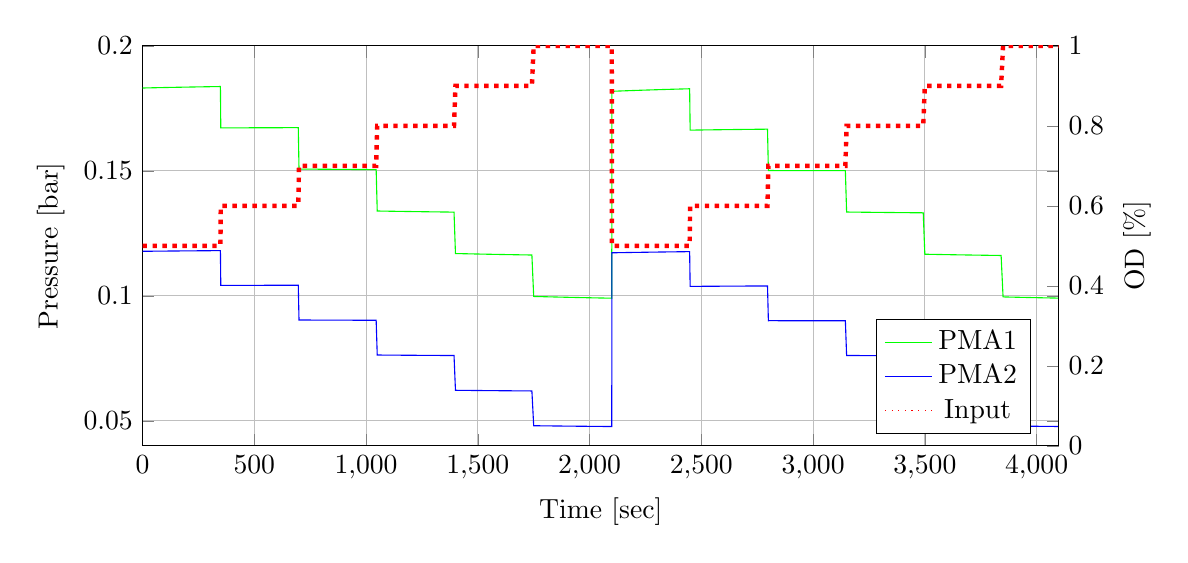
\begin{tikzpicture}

\begin{axis}[%
scaled y ticks = false,
 y tick label style={/pgf/number format/fixed,
/pgf/number format/1000 sep = \thinspace}, % Optional if you want to replace comma as the 1000 separator 
width=4.582in,
height=2in,
at={(0.303in,0.41in)},
scale only axis,
every outer x axis line/.append style={black},
every x tick label/.append style={font=\color{black}},
xmin=0,
xmax=4100,
xlabel={Time [sec]},
xmajorgrids,
every outer y axis line/.append style={black},
every y tick label/.append style={font=\color{black}},
ymin=0.04,
ymax=0.2,
ymajorgrids,
ylabel={Pressure [bar]},
legend pos=south east,
axis background/.style={fill=white}
]
\addplot [color=green,solid]
  table[row sep=crcr]{
0	0.183120331206324\\
8.93323388268949	0.18313855423547\\
17.866467765379	0.183156595942419\\
26.7997016480685	0.183174458131357\\
35.732935530758	0.183192142588518\\
44.6661694134474	0.183209651082365\\
53.5994032961369	0.18322698536376\\
62.5326371788264	0.183244147166147\\
71.4658710615159	0.183261138205721\\
80.3991049442054	0.183277960181601\\
89.3323388268949	0.183294614776\\
98.2655727095844	0.183311103654389\\
107.198806592274	0.183327428465673\\
116.132040474963	0.183343590842346\\
125.065274357653	0.18335959240066\\
133.998508240342	0.183375434740783\\
142.931742123032	0.183391119446965\\
151.864976005721	0.18340664808769\\
160.798209888411	0.183422022215834\\
169.7314437711	0.183437243368823\\
178.66467765379	0.183452313068787\\
187.597911536479	0.183467232822708\\
196.531145419169	0.183482004122575\\
205.464379301858	0.18349662844553\\
214.397613184548	0.183511107254018\\
223.330847067237	0.183525441995933\\
232.264080949927	0.183539634104761\\
241.197314832616	0.183553684999726\\
250.130548715306	0.183567596085928\\
259.063782597995	0.183581368754489\\
267.997016480685	0.183595004382687\\
276.930250363374	0.183608504334097\\
285.863484246064	0.183621869958725\\
294.796718128753	0.183635102593147\\
303.729952011443	0.183648203560636\\
312.663185894132	0.183661174171301\\
321.596419776822	0.183674015722213\\
330.529653659511	0.18368672949754\\
339.462887542201	0.18369931676867\\
348.39612142489	0.18371177879434\\
350	0.167151613191178\\
357.32935530758	0.167163951217602\\
366.262589190269	0.16716705496402\\
375.195823072959	0.167170127827641\\
384.129056955648	0.167173170115753\\
393.062290838338	0.167176182132588\\
401.995524721027	0.16717916417935\\
410.928758603717	0.167182116554247\\
419.861992486406	0.167185039552518\\
428.795226369095	0.167187933466466\\
437.728460251785	0.167190798585485\\
446.661694134474	0.167193635196089\\
455.594928017164	0.167196443581941\\
464.528161899853	0.167199224023884\\
473.461395782543	0.167201976799962\\
482.394629665232	0.167204702185457\\
491.327863547922	0.167207400452908\\
500.261097430611	0.167210071872146\\
509.194331313301	0.167212716710315\\
518.12756519599	0.167215335231899\\
527.06079907868	0.167217927698755\\
535.994032961369	0.167220494370131\\
544.927266844059	0.167223035502696\\
553.860500726748	0.167225551350565\\
562.793734609438	0.167228042165327\\
571.726968492127	0.167230508196063\\
580.660202374817	0.16723294968938\\
589.593436257506	0.167235366889429\\
598.526670140196	0.167237760037932\\
607.459904022885	0.167240129374206\\
616.393137905575	0.167242475135186\\
625.326371788264	0.167244797555451\\
634.259605670954	0.167247096867245\\
643.192839553643	0.167249373300501\\
652.126073436333	0.167251627082864\\
661.059307319022	0.167253858439714\\
669.992541201712	0.16725606759419\\
678.925775084401	0.167258254767207\\
687.859008967091	0.167260420177487\\
696.79224284978	0.167262564041571\\
700	0.150702398438409\\
705.72547673247	0.150704520970685\\
714.658710615159	0.150697510868836\\
723.591944497849	0.150690570518677\\
732.525178380538	0.150683699226166\\
741.458412263228	0.150676896304168\\
750.391646145917	0.150670161072386\\
759.324880028607	0.150663492857289\\
768.258113911296	0.150656890992052\\
777.191347793986	0.150650354816481\\
786.124581676675	0.150643883676953\\
795.057815559364	0.15063747692635\\
803.991049442054	0.150631133923989\\
812.924283324744	0.150624854035567\\
821.857517207433	0.150618636633087\\
830.790751090123	0.150612481094806\\
839.723984972812	0.150606386805162\\
848.657218855501	0.150600353154724\\
857.590452738191	0.150594379540119\\
866.52368662088	0.150588465363982\\
875.45692050357	0.150582610034889\\
884.390154386259	0.150576812967303\\
893.323388268949	0.150571073581513\\
902.256622151638	0.150565391303573\\
911.189856034328	0.150559765565253\\
920.123089917017	0.150554195803972\\
929.056323799707	0.150548681462751\\
937.989557682396	0.15054322199015\\
946.922791565086	0.150537816840217\\
955.856025447775	0.150532465472432\\
964.789259330465	0.150527167351655\\
973.722493213154	0.150521921948069\\
982.655727095844	0.150516728737128\\
991.588960978533	0.150511587199507\\
1000.52219486122	0.150506496821048\\
1009.45542874391	0.150501457092709\\
1018.3886626266	0.150496467510512\\
1027.32189650929	0.150491527575495\\
1036.25513039198	0.15048663679366\\
1045.18836427467	0.150481794675925\\
1050	0.133921629072763\\
1054.12159815736	0.133916835134912\\
1063.05483204005	0.133902977382973\\
1071.98806592274	0.133889257517991\\
1080.92129980543	0.133875674167968\\
1089.85453368812	0.133862225974555\\
1098.78776757081	0.133848911592924\\
1107.7210014535	0.133835729691623\\
1116.65423533619	0.133822678952451\\
1125.58746921888	0.133809758070324\\
1134.52070310157	0.133796965753141\\
1143.45393698425	0.133784300721661\\
1152.38717086694	0.133771761709368\\
1161.32040474963	0.133759347462351\\
1170.25363863232	0.133747056739175\\
1179.18687251501	0.133734888310756\\
1188.1201063977	0.133722840960242\\
1197.05334028039	0.133710913482886\\
1205.98657416308	0.13369910468593\\
1214.91980804577	0.133687413388485\\
1223.85304192846	0.133675838421412\\
1232.78627581115	0.133664378627202\\
1241.71950969384	0.133653032859868\\
1250.65274357653	0.133641799984821\\
1259.58597745922	0.133630678878766\\
1268.51921134191	0.133619668429582\\
1277.4524452246	0.133608767536214\\
1286.38567910729	0.133597975108564\\
1295.31891298998	0.13358729006738\\
1304.25214687267	0.133576711344148\\
1313.18538075535	0.133566237880986\\
1322.11861463804	0.133555868630541\\
1331.05184852073	0.133545602555877\\
1339.98508240342	0.133535438630377\\
1348.91831628611	0.133525375837642\\
1357.8515501688	0.133515413171383\\
1366.78478405149	0.133505549635324\\
1375.71801793418	0.133495784243104\\
1384.65125181687	0.133486116018174\\
1393.58448569956	0.133476543993705\\
1400	0.116916378390543\\
1402.51771958225	0.116906901609322\\
1411.45095346494	0.116888407609092\\
1420.38418734763	0.116870097627267\\
1429.31742123032	0.116851969832832\\
1438.25065511301	0.116834022412993\\
1447.1838889957	0.116816253572993\\
1456.11712287839	0.116798661535931\\
1465.05035676108	0.11678124454259\\
1473.98359064377	0.116764000851254\\
1482.91682452646	0.116746928737539\\
1491.85005840914	0.11673002649422\\
1500.78329229183	0.116713292431058\\
1509.71652617452	0.116696724874631\\
1518.64976005721	0.11668032216817\\
1527.5829939399	0.11666408267139\\
1536.51622782259	0.116648004760328\\
1545.44946170528	0.116632086827178\\
1554.38269558797	0.116616327280133\\
1563.31592947066	0.116600724543225\\
1572.24916335335	0.116585277056166\\
1581.18239723604	0.116569983274196\\
1590.11563111873	0.116554841667921\\
1599.04886500142	0.11653985072317\\
1607.98209888411	0.116525008940833\\
1616.9153327668	0.116510314836721\\
1625.84856664949	0.116495766941409\\
1634.78180053218	0.116481363800097\\
1643.71503441487	0.116467103972456\\
1652.64826829756	0.116452986032493\\
1661.58150218025	0.116439008568401\\
1670.51473606293	0.116425170182422\\
1679.44796994562	0.116411469490705\\
1688.38120382831	0.116397905123168\\
1697.314437711	0.116384475723365\\
1706.24767159369	0.116371179948342\\
1715.18090547638	0.116358016468511\\
1724.11413935907	0.116344983967513\\
1733.04737324176	0.116332081142086\\
1741.98060712445	0.116319306701936\\
1750	0.0997591410987745\\
1750.91384100714	0.0997464937664476\\
1759.84707488983	0.0997248607626262\\
1768.78030877252	0.0997034430108219\\
1777.71354265521	0.0996822383692411\\
1786.6467765379	0.0996612447174013\\
1795.58001042059	0.0996404599559192\\
1804.51324430328	0.0996198820063007\\
1813.44647818597	0.0995995088107331\\
1822.37971206866	0.0995793383318792\\
1831.31294595135	0.0995593685526737\\
1840.24617983403	0.0995395974761213\\
1849.17941371672	0.0995200231250975\\
1858.11264759941	0.0995006435421502\\
1867.0458814821	0.0994814567893043\\
1875.97911536479	0.099462460947868\\
1884.91234924748	0.0994436541182408\\
1893.84558313017	0.0994250344197233\\
1902.77881701286	0.0994065999903298\\
1911.71205089555	0.0993883489866012\\
1920.64528477824	0.0993702795834216\\
1929.57851866093	0.0993523899738349\\
1938.51175254362	0.0993346783688648\\
1947.44498642631	0.0993171429973354\\
1956.378220309	0.0992997821056945\\
1965.31145419169	0.0992825939578378\\
1974.24468807438	0.0992655768349358\\
1983.17792195707	0.0992487290352615\\
1992.11115583976	0.0992320488740204\\
2001.04438972245	0.0992155346831818\\
2009.97762360514	0.0991991848113125\\
2018.91085748782	0.0991829976234112\\
2027.84409137051	0.099166971500745\\
2036.7773252532	0.0991511048406879\\
2045.71055913589	0.0991353960565602\\
2054.64379301858	0.0991198435774698\\
2063.57702690127	0.0991044458481555\\
2072.51026078396	0.099089201328831\\
2081.44349466665	0.0990741084950312\\
2090.37672854934	0.0990591658374596\\
2099.30996243203	0.0990443718618377\\
2100	0.181845199877648\\
2108.24319631472	0.181830553104565\\
2117.17643019741	0.181861609642197\\
2126.1096640801	0.181892357162069\\
2135.04289796279	0.18192279873896\\
2143.97613184548	0.181952937417054\\
2152.90936572817	0.181982776210245\\
2161.84259961086	0.182012318102439\\
2170.77583349355	0.182041566047848\\
2179.70906737624	0.182070522971295\\
2188.64230125892	0.182099191768495\\
2197.57553514161	0.182127575306354\\
2206.5087690243	0.182155676423249\\
2215.44200290699	0.182183497929317\\
2224.37523678968	0.182211042606733\\
2233.30847067237	0.182238313209987\\
2242.24170455506	0.182265312466164\\
2251.17493843775	0.182292043075212\\
2260.10817232044	0.182318507710216\\
2269.04140620313	0.182344709017663\\
2277.97464008582	0.182370649617704\\
2286.90787396851	0.182396332104423\\
2295.8411078512	0.182421759046091\\
2304.77434173389	0.182446932985424\\
2313.70757561658	0.182471856439837\\
2322.64080949927	0.182496531901698\\
2331.57404338196	0.182520961838574\\
2340.50727726465	0.182545148693479\\
2349.44051114734	0.18256909488512\\
2358.37374503003	0.182592802808138\\
2367.30697891271	0.182616274833344\\
2376.2402127954	0.182639513307961\\
2385.17344667809	0.182662520555858\\
2394.10668056078	0.182685298877778\\
2403.03991444347	0.182707850551574\\
2411.97314832616	0.182730177832433\\
2420.90638220885	0.182752282953101\\
2429.83961609154	0.182774168124111\\
2438.77284997423	0.182795835533997\\
2447.70608385692	0.18281728734952\\
2450	0.166257121746358\\
2456.63931773961	0.166278360112718\\
2465.5725516223	0.166290275639196\\
2474.50578550499	0.166302072604188\\
2483.43901938768	0.166313752187398\\
2492.37225327037	0.166325315556796\\
2501.30548715306	0.166336763868729\\
2510.23872103575	0.166348098268037\\
2519.17195491844	0.166359319888171\\
2528.10518880113	0.166370429851302\\
2537.03842268382	0.166381429268436\\
2545.9716565665	0.166392319239525\\
2554.90489044919	0.166403100853574\\
2563.83812433188	0.166413775188754\\
2572.77135821457	0.166424343312509\\
2581.70459209726	0.16643480628166\\
2590.63782597995	0.166445165142512\\
2599.57105986264	0.166455420930961\\
2608.50429374533	0.166465574672594\\
2617.43752762802	0.166475627382795\\
2626.37076151071	0.166485580066843\\
2635.3039953934	0.166495433720015\\
2644.23722927609	0.166505189327684\\
2653.17046315878	0.166514847865421\\
2662.10369704147	0.166524410299087\\
2671.03693092416	0.166533877584934\\
2679.97016480685	0.166543250669698\\
2688.90339868954	0.166552530490697\\
2697.83663257223	0.16656171797592\\
2706.76986645492	0.166570814044124\\
2715.7031003376	0.166579819604923\\
2724.63633422029	0.166588735558881\\
2733.56956810298	0.166597562797602\\
2742.50280198567	0.166606302203816\\
2751.43603586836	0.166614954651473\\
2760.36926975105	0.166623521005824\\
2769.30250363374	0.166632002123512\\
2778.23573751643	0.166640398852656\\
2787.16897139912	0.166648712032937\\
2796.10220528181	0.166656942495679\\
2800	0.150096776892517\\
2805.0354391645	0.150104925460774\\
2813.96867304719	0.150103881434837\\
2822.90190692988	0.150102847797133\\
2831.83514081257	0.150101824444298\\
2840.76837469526	0.150100811273995\\
2849.70160857795	0.150099808184907\\
2858.63484246064	0.150098815076723\\
2867.56807634333	0.150097831850133\\
2876.50131022602	0.150096858406811\\
2885.4345441087	0.150095894649415\\
2894.36777799139	0.150094940481566\\
2903.30101187408	0.150093995807847\\
2912.23424575677	0.15009306053379\\
2921.16747963946	0.150092134565867\\
2930.10071352215	0.15009121781148\\
2939.03394740484	0.150090310178953\\
2947.96718128753	0.150089411577522\\
2956.90041517022	0.150088521917326\\
2965.83364905291	0.150087641109398\\
2974.7668829356	0.150086769065657\\
2983.70011681829	0.150085905698898\\
2992.63335070098	0.150085050922782\\
3001.56658458367	0.150084204651832\\
3010.49981846636	0.15008336680142\\
3019.43305234905	0.150082537287761\\
3028.36628623174	0.150081716027901\\
3037.29952011443	0.150080902939715\\
3046.23275399712	0.150080097941892\\
3055.16598787981	0.150079300953933\\
3064.09922176249	0.150078511896138\\
3073.03245564518	0.1500777306896\\
3081.96568952787	0.150076957256199\\
3090.89892341056	0.150076191518589\\
3099.83215729325	0.150075433400197\\
3108.76539117594	0.150074682825211\\
3117.69862505863	0.150073939718571\\
3126.63185894132	0.150073204005967\\
3135.56509282401	0.150072475613827\\
3144.4983267067	0.150071754469311\\
3150	0.133511588866149\\
3153.43156058939	0.133510874897142\\
3162.36479447208	0.133501056517673\\
3171.29802835477	0.133491335832727\\
3180.23126223746	0.133481711870227\\
3189.16449612015	0.133472183667768\\
3198.09773000284	0.133462750272523\\
3207.03096388553	0.133453410741142\\
3215.96419776822	0.133444164139666\\
3224.89743165091	0.133435009543425\\
3233.8306655336	0.133425946036953\\
3242.76389941628	0.133416972713891\\
3251.69713329897	0.133408088676899\\
3260.63036718166	0.133399293037565\\
3269.56360106435	0.133390584916318\\
3278.49683494704	0.133381963442338\\
3287.43006882973	0.133373427753471\\
3296.36330271242	0.13336497699614\\
3305.29653659511	0.133356610325262\\
3314.2297704778	0.133348326904163\\
3323.16300436049	0.133340125904493\\
3332.09623824318	0.133332006506146\\
3341.02947212587	0.133323967897174\\
3349.96270600856	0.133316009273711\\
3358.89593989125	0.133308129839886\\
3367.82917377394	0.133300328807749\\
3376.76240765663	0.133292605397191\\
3385.69564153932	0.133284958835864\\
3394.62887542201	0.133277388359104\\
3403.5621093047	0.133269893209859\\
3412.49534318738	0.133262472638606\\
3421.42857707007	0.133255125903281\\
3430.36181095276	0.133247852269206\\
3439.29504483545	0.13324065100901\\
3448.22827871814	0.133233521402561\\
3457.16151260083	0.133226462736892\\
3466.09474648352	0.13321947430613\\
3475.02798036621	0.133212555411428\\
3483.9612142489	0.133205705360888\\
3492.89444813159	0.1331989234695\\
3500	0.116638757866338\\
3501.82768201428	0.116632043455907\\
3510.76091589697	0.116616284340414\\
3519.69414977966	0.116600682030763\\
3528.62738366235	0.116585234966711\\
3537.56061754504	0.116569941603537\\
3546.49385142773	0.116554800411893\\
3555.42708531042	0.116539809877646\\
3564.36031919311	0.116524968501729\\
3573.2935530758	0.116510274799992\\
3582.22678695849	0.116495727303053\\
3591.16002084117	0.116481324556149\\
3600.09325472386	0.116467065118992\\
3609.02648860655	0.116452947565628\\
3617.95972248924	0.116438970484288\\
3626.89295637193	0.116425132477252\\
3635.82619025462	0.116411432160707\\
3644.75942413731	0.116397868164611\\
3653.69265802	0.116384439132551\\
3662.62589190269	0.116371143721613\\
3671.55912578538	0.116357980602244\\
3680.49235966807	0.116344948458121\\
3689.42559355076	0.116332045986018\\
3698.35882743345	0.116319271895678\\
3707.29206131614	0.116306624909679\\
3716.22529519883	0.116294103763313\\
3725.15852908152	0.116281707204453\\
3734.09176296421	0.116269433993434\\
3743.0249968469	0.116257282902923\\
3751.95823072959	0.116245252717802\\
3760.89146461227	0.11623334223504\\
3769.82469849496	0.116221550263581\\
3778.75793237765	0.116209875624215\\
3787.69116626034	0.11619831714947\\
3796.62440014303	0.116186873683487\\
3805.55763402572	0.116175544081911\\
3814.49086790841	0.116164327211771\\
3823.4241017911	0.11615322195137\\
3832.35733567379	0.116142227190174\\
3841.29056955648	0.116131341828696\\
3850	0.0995711762255341\\
3850.22380343917	0.099560399175229\\
3859.15703732186	0.0995406178438094\\
3868.09027120455	0.0995210333399559\\
3877.02350508724	0.0995016437052012\\
3885.95673896993	0.0994824470005652\\
3894.88997285262	0.0994634413063608\\
3903.82320673531	0.099444624722002\\
3912.756440618	0.0994259953658143\\
3921.68967450069	0.099407551374846\\
3930.62290838338	0.0993892909046819\\
3939.55614226606	0.0993712121292593\\
3948.48937614875	0.0993533132406851\\
3957.42261003144	0.0993355924490549\\
3966.35584391413	0.0993180479822743\\
3975.28907779682	0.0993006780858814\\
3984.22231167951	0.0992834810228716\\
3993.1555455622	0.0992664550735237\\
4002.08877944489	0.0992495985352281\\
4011.02201332758	0.0992329097223164\\
4019.95524721027	0.0992163869658929\\
4028.88848109296	0.0992000286136677\\
4037.82171497565	0.0991838330297913\\
4046.75494885834	0.0991677985946915\\
4055.68818274103	0.0991519237049109\\
4064.62141662372	0.0991362067729468\\
4073.55465050641	0.0991206462270924\\
4082.4878843891	0.0991052405112797\\
4091.42111827179	0.0990899880849238\\
4100	0.0990899880849238\\
};
\addlegendentry{PMA1};

\addplot [color=blue,solid]
  table[row sep=crcr]{
0	0.117805105096511\\
8.93323388268949	0.117813362210315\\
17.866467765379	0.117821537164452\\
26.7997016480685	0.117829630776424\\
35.732935530758	0.117837643855598\\
44.6661694134474	0.117845577203291\\
53.5994032961369	0.117853431612843\\
62.5326371788264	0.117861207869702\\
71.4658710615159	0.117868906751502\\
80.3991049442054	0.117876529028135\\
89.3323388268949	0.117884075461838\\
98.2655727095844	0.117891546807259\\
107.198806592274	0.11789894381154\\
116.132040474963	0.117906267214387\\
125.065274357653	0.117913517748147\\
133.998508240342	0.117920696137881\\
142.931742123032	0.117927803101432\\
151.864976005721	0.117934839349503\\
160.798209888411	0.117941805585726\\
169.7314437711	0.117948702506729\\
178.66467765379	0.117955530802212\\
187.597911536479	0.117962291155009\\
196.531145419169	0.117968984241162\\
205.464379301858	0.117975610729984\\
214.397613184548	0.117982171284132\\
223.330847067237	0.117988666559664\\
232.264080949927	0.117995097206116\\
241.197314832616	0.118001463866556\\
250.130548715306	0.118007767177658\\
259.063782597995	0.118014007769756\\
267.997016480685	0.118020186266916\\
276.930250363374	0.118026303286992\\
285.863484246064	0.118032359441693\\
294.796718128753	0.118038355336639\\
303.729952011443	0.118044291571423\\
312.663185894132	0.118050168739676\\
321.596419776822	0.118055987429119\\
330.529653659511	0.118061748221626\\
339.462887542201	0.118067451693281\\
348.39612142489	0.118073098414436\\
350	0.10417054586618\\
357.32935530758	0.104176136401513\\
366.262589190269	0.104177542753179\\
375.195823072959	0.104178935111409\\
384.129056955648	0.104180313615442\\
393.062290838338	0.104181678403129\\
401.995524721027	0.104183029610949\\
410.928758603717	0.104184367374024\\
419.861992486406	0.104185691826132\\
428.795226369095	0.10418700309972\\
437.728460251785	0.104188301325916\\
446.661694134474	0.104189586634543\\
455.594928017164	0.104190859154134\\
464.528161899853	0.104192119011941\\
473.461395782543	0.104193366333952\\
482.394629665232	0.104194601244899\\
491.327863547922	0.104195823868276\\
500.261097430611	0.104197034326345\\
509.194331313301	0.104198232740152\\
518.12756519599	0.104199419229542\\
527.06079907868	0.104200593913163\\
535.994032961369	0.104201756908485\\
544.927266844059	0.104202908331808\\
553.860500726748	0.104204048298276\\
562.793734609438	0.104205176921887\\
571.726968492127	0.104206294315503\\
580.660202374817	0.104207400590865\\
589.593436257506	0.104208495858602\\
598.526670140196	0.104209580228241\\
607.459904022885	0.10421065380822\\
616.393137905575	0.104211716705899\\
625.326371788264	0.104212769027567\\
634.259605670954	0.104213810878458\\
643.192839553643	0.104214842362758\\
652.126073436333	0.104215863583616\\
661.059307319022	0.104216874643155\\
669.992541201712	0.104217875642482\\
678.925775084401	0.104218866681698\\
687.859008967091	0.104219847859908\\
696.79224284978	0.104220819275229\\
700	0.0903182667269739\\
705.72547673247	0.0903192284765502\\
714.658710615159	0.0903160520996548\\
723.591944497849	0.0903129073282423\\
732.525178380538	0.090309793847833\\
741.458412263228	0.0903067113470761\\
750.391646145917	0.0903036595177188\\
759.324880028607	0.0903006380545755\\
768.258113911296	0.0902976466554975\\
777.191347793986	0.0902946850213421\\
786.124581676675	0.0902917528559434\\
795.057815559364	0.0902888498660823\\
803.991049442054	0.0902859757614573\\
812.924283324744	0.0902831302546555\\
821.857517207433	0.0902803130611238\\
830.790751090123	0.0902775238991403\\
839.723984972812	0.0902747624897864\\
848.657218855501	0.0902720285569189\\
857.590452738191	0.0902693218271421\\
866.52368662088	0.0902666420297806\\
875.45692050357	0.0902639888968524\\
884.390154386259	0.090261362163042\\
893.323388268949	0.0902587615656736\\
902.256622151638	0.0902561868446853\\
911.189856034328	0.0902536377426028\\
920.123089917017	0.0902511140045136\\
929.056323799707	0.0902486153780418\\
937.989557682396	0.0902461416133226\\
946.922791565086	0.0902436924629773\\
955.856025447775	0.0902412676820889\\
964.789259330465	0.090238867028177\\
973.722493213154	0.0902364902611743\\
982.655727095844	0.090234137143402\\
991.588960978533	0.0902318074395463\\
1000.52219486122	0.0902295009166348\\
1009.45542874391	0.0902272173440133\\
1018.3886626266	0.0902249564933224\\
1027.32189650929	0.0902227181384751\\
1036.25513039198	0.0902205020556341\\
1045.18836427467	0.0902183080231891\\
1050	0.0763157554749336\\
1054.12159815736	0.0763135832734795\\
1063.05483204005	0.0763073041288922\\
1071.98806592274	0.0763010874628469\\
1080.92129980543	0.0762949326536717\\
1089.85453368812	0.0762888390858803\\
1098.78776757081	0.0762828061501106\\
1107.7210014535	0.076276833243064\\
1116.65423533619	0.0762709197674445\\
1125.58746921888	0.0762650651318995\\
1134.52070310157	0.0762592687509603\\
1143.45393698425	0.0762535300449839\\
1152.38717086694	0.0762478484400946\\
1161.32040474963	0.0762422233681271\\
1170.25363863232	0.0762366542665694\\
1179.18687251501	0.0762311405785065\\
1188.1201063977	0.0762256817525647\\
1197.05334028039	0.0762202772428569\\
1205.98657416308	0.0762149265089273\\
1214.91980804577	0.0762096290156979\\
1223.85304192846	0.0762043842334149\\
1232.78627581115	0.0761991916375954\\
1241.71950969384	0.0761940507089755\\
1250.65274357653	0.0761889609334578\\
1259.58597745922	0.0761839218020603\\
1268.51921134191	0.0761789328108657\\
1277.4524452246	0.0761739934609703\\
1286.38567910729	0.076169103258435\\
1295.31891298998	0.0761642617142354\\
1304.25214687267	0.0761594683442127\\
1313.18538075535	0.0761547226690259\\
1322.11861463804	0.0761500242141034\\
1331.05184852073	0.0761453725095955\\
1339.98508240342	0.0761407670903279\\
1348.91831628611	0.0761362074957546\\
1357.8515501688	0.0761316932699122\\
1366.78478405149	0.0761272239613742\\
1375.71801793418	0.076122799123206\\
1384.65125181687	0.0761184183129199\\
1393.58448569956	0.076114081092431\\
1400	0.0622115285441754\\
1402.51771958225	0.062207234479758\\
1411.45095346494	0.0621988545850998\\
1420.38418734763	0.0621905580717993\\
1429.31742123032	0.062182344110198\\
1438.25065511301	0.0621742118788925\\
1447.1838889957	0.0621661605646528\\
1456.11712287839	0.0621581893623405\\
1465.05035676108	0.0621502974748284\\
1473.98359064377	0.062142484112921\\
1482.91682452646	0.0621347484952754\\
1491.85005840914	0.0621270898483231\\
1500.78329229183	0.0621195074061927\\
1509.71652617452	0.0621120004106336\\
1518.64976005721	0.0621045681109397\\
1527.5829939399	0.0620972097638745\\
1536.51622782259	0.0620899246335971\\
1545.44946170528	0.0620827119915882\\
1554.38269558797	0.0620755711165772\\
1563.31592947066	0.0620685012944705\\
1572.24916335335	0.0620615018182798\\
1581.18239723604	0.0620545719880514\\
1590.11563111873	0.0620477111107964\\
1599.04886500142	0.062040918500421\\
1607.98209888411	0.0620341934776584\\
1616.9153327668	0.0620275353700004\\
1625.84856664949	0.0620209435116307\\
1634.78180053218	0.0620144172433575\\
1643.71503441487	0.0620079559125485\\
1652.64826829756	0.062001558873065\\
1661.58150218025	0.0619952254851976\\
1670.51473606293	0.0619889551156019\\
1679.44796994562	0.0619827471372356\\
1688.38120382831	0.0619766009292955\\
1697.314437711	0.0619705158771555\\
1706.24767159369	0.0619644913723051\\
1715.18090547638	0.0619585268122887\\
1724.11413935907	0.061952621600645\\
1733.04737324176	0.0619467751468479\\
1741.98060712445	0.0619409868662468\\
1750	0.0480384343179912\\
1750.91384100714	0.0480327036317532\\
1759.84707488983	0.0480229014099025\\
1768.78030877252	0.0480131967218036\\
1777.71354265521	0.0480035885969794\\
1786.6467765379	0.047994076074609\\
1795.58001042059	0.047984658203432\\
1804.51324430328	0.0479753340416532\\
1813.44647818597	0.0479661026568483\\
1822.37971206866	0.0479569631258709\\
1831.31294595135	0.0479479145347599\\
1840.24617983403	0.0479389559786485\\
1849.17941371672	0.0479300865616733\\
1858.11264759941	0.0479213053968849\\
1867.0458814821	0.0479126116061593\\
1875.97911536479	0.0479040043201099\\
1884.91234924748	0.0478954826780006\\
1893.84558313017	0.0478870458276599\\
1902.77881701286	0.0478786929253955\\
1911.71205089555	0.0478704231359099\\
1920.64528477824	0.047862235632217\\
1929.57851866093	0.0478541295955594\\
1938.51175254362	0.0478461042153263\\
1947.44498642631	0.047838158688973\\
1956.378220309	0.0478302922219398\\
1965.31145419169	0.0478225040275733\\
1974.24468807438	0.0478147933270472\\
1983.17792195707	0.047807159349285\\
1992.11115583976	0.0477996013308821\\
2001.04438972245	0.0477921185160303\\
2009.97762360514	0.0477847101564416\\
2018.91085748782	0.0477773755112736\\
2027.84409137051	0.0477701138470555\\
2036.7773252532	0.0477629244376146\\
2045.71055913589	0.0477558065640037\\
2054.64379301858	0.0477487595144293\\
2063.57702690127	0.0477417825841805\\
2072.51026078396	0.047734875075558\\
2081.44349466665	0.0477280362978052\\
2090.37672854934	0.0477212655670382\\
2099.30996243203	0.0477145622061783\\
2100	0.117227324947456\\
2108.24319631472	0.117220688286161\\
2117.17643019741	0.11723476044527\\
2126.1096640801	0.117248692584035\\
2135.04289796279	0.117262486095682\\
2143.97613184548	0.117276142359574\\
2152.90936572817	0.11728966274135\\
2161.84259961086	0.117303048593059\\
2170.77583349355	0.117316301253297\\
2179.70906737624	0.117329422047343\\
2188.64230125892	0.117342412287287\\
2197.57553514161	0.117355273272165\\
2206.5087690243	0.117368006288085\\
2215.44200290699	0.11738061260836\\
2224.37523678968	0.117393093493635\\
2233.30847067237	0.117405450192007\\
2242.24170455506	0.117417683939157\\
2251.17493843775	0.11742979595847\\
2260.10817232044	0.11744178746116\\
2269.04140620313	0.117453659646386\\
2277.97464008582	0.117465413701377\\
2286.90787396851	0.11747705080155\\
2295.8411078512	0.117488572110623\\
2304.77434173389	0.117499978780739\\
2313.70757561658	0.117511271952573\\
2322.64080949927	0.117522452755453\\
2331.57404338196	0.117533522307468\\
2340.50727726465	0.117544481715584\\
2349.44051114734	0.117555332075751\\
2358.37374503003	0.117566074473013\\
2367.30697891271	0.117576709981621\\
2376.2402127954	0.117587239665134\\
2385.17344667809	0.11759766457653\\
2394.10668056078	0.117607985758308\\
2403.03991444347	0.117618204242596\\
2411.97314832616	0.117628321051251\\
2420.90638220885	0.117638337195963\\
2429.83961609154	0.117648253678355\\
2438.77284997423	0.117658071490083\\
2447.70608385692	0.117667791612937\\
2450	0.103765239064682\\
2456.63931773961	0.103774862470683\\
2465.5725516223	0.103780261565279\\
2474.50578550499	0.103785606937977\\
2483.43901938768	0.10379089912332\\
2492.37225327037	0.103796138650531\\
2501.30548715306	0.103801326043568\\
2510.23872103575	0.103806461821173\\
2519.17195491844	0.10381154649693\\
2528.10518880113	0.10381658057931\\
2537.03842268382	0.103821564571726\\
2545.9716565665	0.103826498972581\\
2554.90489044919	0.10383138427532\\
2563.83812433188	0.103836220968477\\
2572.77135821457	0.103841009535725\\
2581.70459209726	0.103845750455927\\
2590.63782597995	0.103850444203177\\
2599.57105986264	0.103855091246854\\
2608.50429374533	0.103859692051667\\
2617.43752762802	0.1038642470777\\
2626.37076151071	0.103868756780461\\
2635.3039953934	0.103873221610922\\
2644.23722927609	0.103877642015571\\
2653.17046315878	0.103882018436452\\
2662.10369704147	0.103886351311212\\
2671.03693092416	0.10389064107314\\
2679.97016480685	0.103894888151218\\
2688.90339868954	0.103899092970157\\
2697.83663257223	0.103903255950441\\
2706.76986645492	0.103907377508373\\
2715.7031003376	0.103911458056113\\
2724.63633422029	0.103915498001718\\
2733.56956810298	0.103919497749186\\
2742.50280198567	0.103923457698496\\
2751.43603586836	0.103927378245647\\
2760.36926975105	0.103931259782695\\
2769.30250363374	0.103935102697798\\
2778.23573751643	0.103938907375252\\
2787.16897139912	0.103942674195527\\
2796.10220528181	0.103946403535308\\
2800	0.090043850987052\\
2805.0354391645	0.0900475432192765\\
2813.96867304719	0.0900470701562689\\
2822.90190692988	0.0900466018003175\\
2831.83514081257	0.0900461381045864\\
2840.76837469526	0.0900456790227057\\
2849.70160857795	0.0900452245087666\\
2858.63484246064	0.0900447745173175\\
2867.56807634333	0.0900443290033589\\
2876.50131022602	0.0900438879223388\\
2885.4345441087	0.0900434512301489\\
2894.36777799139	0.0900430188831195\\
2903.30101187408	0.0900425908380157\\
2912.23424575677	0.0900421670520324\\
2921.16747963946	0.0900417474827907\\
2930.10071352215	0.0900413320883334\\
2939.03394740484	0.0900409208271206\\
2947.96718128753	0.0900405136580259\\
2956.90041517022	0.0900401105403319\\
2965.83364905291	0.0900397114337267\\
2974.7668829356	0.0900393162982991\\
2983.70011681829	0.0900389250945353\\
2992.63335070098	0.0900385377833146\\
3001.56658458367	0.0900381543259056\\
3010.49981846636	0.090037774683962\\
3019.43305234905	0.0900373988195195\\
3028.36628623174	0.0900370266949913\\
3037.29952011443	0.0900366582731645\\
3046.23275399712	0.0900362935171967\\
3055.16598787981	0.090035932390612\\
3064.09922176249	0.0900355748572974\\
3073.03245564518	0.0900352208814993\\
3081.96568952787	0.0900348704278197\\
3090.89892341056	0.090034523461213\\
3099.83215729325	0.0900341799469823\\
3108.76539117594	0.0900338398507758\\
3117.69862505863	0.0900335031385836\\
3126.63185894132	0.0900331697767342\\
3135.56509282401	0.0900328397318912\\
3144.4983267067	0.0900325129710497\\
3150	0.0761299604227941\\
3153.43156058939	0.0761296369132778\\
3162.36479447208	0.0761251880658333\\
3171.29802835477	0.0761207834851673\\
3180.23126223746	0.0761164227308177\\
3189.16449612015	0.0761121053667056\\
3198.09773000284	0.0761078309610906\\
3207.03096388553	0.0761035990865285\\
3215.96419776822	0.0760994093198283\\
3224.89743165091	0.0760952612420097\\
3233.8306655336	0.0760911544382612\\
3242.76389941628	0.0760870884978989\\
3251.69713329897	0.0760830630143254\\
3260.63036718166	0.0760790775849888\\
3269.56360106435	0.0760751318113426\\
3278.49683494704	0.0760712252988062\\
3287.43006882973	0.0760673576567248\\
3296.36330271242	0.076063528498331\\
3305.29653659511	0.0760597374407056\\
3314.2297704778	0.0760559841047396\\
3323.16300436049	0.0760522681150961\\
3332.09623824318	0.0760485891001729\\
3341.02947212587	0.0760449466920654\\
3349.96270600856	0.0760413405265296\\
3358.89593989125	0.0760377702429459\\
3367.82917377394	0.0760342354842828\\
3376.76240765663	0.0760307358970613\\
3385.69564153932	0.0760272711313199\\
3394.62887542201	0.0760238408405787\\
3403.5621093047	0.076020444681806\\
3412.49534318738	0.0760170823153827\\
3421.42857707007	0.0760137534050695\\
3430.36181095276	0.0760104576179723\\
3439.29504483545	0.0760071946245096\\
3448.22827871814	0.0760039640983793\\
3457.16151260083	0.076000765716526\\
3466.09474648352	0.0759975991591086\\
3475.02798036621	0.0759944641094688\\
3483.9612142489	0.0759913602540988\\
3492.89444813159	0.0759882872826104\\
3500	0.0620857347343549\\
3501.82768201428	0.0620826923394484\\
3510.76091589697	0.0620755516599795\\
3519.69414977966	0.0620684820314692\\
3528.62738366235	0.0620614827469486\\
3537.56061754504	0.0620545531064832\\
3546.49385142773	0.0620476924171029\\
3555.42708531042	0.0620408999927329\\
3564.36031919311	0.0620341751541249\\
3573.2935530758	0.0620275172287892\\
3582.22678695849	0.0620209255509275\\
3591.16002084117	0.0620143994613664\\
3600.09325472386	0.0620079383074912\\
3609.02648860655	0.062001541443181\\
3617.95972248924	0.0619952082287438\\
3626.89295637193	0.0619889380308527\\
3635.82619025462	0.0619827302224825\\
3644.75942413731	0.0619765841828471\\
3653.69265802	0.061970499297337\\
3662.62589190269	0.0619644749574586\\
3671.55912578538	0.0619585105607727\\
3680.49235966807	0.0619526055108343\\
3689.42559355076	0.0619467592171335\\
3698.35882743345	0.0619409710950357\\
3707.29206131614	0.0619352405657239\\
3716.22529519883	0.06192956705614\\
3725.15852908152	0.0619239499989283\\
3734.09176296421	0.0619183888323782\\
3743.0249968469	0.0619128830003682\\
3751.95823072959	0.0619074319523103\\
3760.89146461227	0.0619020351430951\\
3769.82469849496	0.061896692033037\\
3778.75793237765	0.0618914020878202\\
3787.69116626034	0.0618861647784459\\
3796.62440014303	0.0618809795811784\\
3805.55763402572	0.0618758459774936\\
3814.49086790841	0.0618707634540267\\
3823.4241017911	0.0618657315025209\\
3832.35733567379	0.0618607496197767\\
3841.29056955648	0.0618558173076017\\
3850	0.0479532647593461\\
3850.22380343917	0.0479483815245046\\
3859.15703732186	0.0479394183217669\\
3868.09027120455	0.0479305443044001\\
3877.02350508724	0.0479217585849948\\
3885.95673896993	0.0479130602849715\\
3894.88997285262	0.0479044485344926\\
3903.82320673531	0.0478959224723757\\
3912.756440618	0.0478874812460072\\
3921.68967450069	0.0478791240112572\\
3930.62290838338	0.0478708499323949\\
3939.55614226606	0.0478626581820054\\
3948.48937614875	0.0478545479409065\\
3957.42261003144	0.0478465183980671\\
3966.35584391413	0.047838568750526\\
3975.28907779682	0.0478306982033115\\
3984.22231167951	0.0478229059693622\\
3993.1555455622	0.047815191269448\\
4002.08877944489	0.0478075533320921\\
4011.02201332758	0.0477999913934942\\
4019.95524721027	0.047792504697454\\
4028.88848109296	0.0477850924952953\\
4037.82171497565	0.0477777540457916\\
4046.75494885834	0.0477704886150915\\
4055.68818274103	0.0477632954766458\\
4064.62141662372	0.0477561739111343\\
4073.55465050641	0.0477491232063944\\
4082.4878843891	0.0477421426573494\\
4091.42111827179	0.0477352315659385\\
4100	0.0477352315659385\\
};
\addlegendentry{PMA2};
\addplot [color=red,dotted]
  table[row sep=crcr]{
0	0\\
};
\addlegendentry{Input};

\end{axis}

\begin{axis}[
scaled y ticks = false,
 y tick label style={/pgf/number format/fixed,
/pgf/number format/1000 sep = \thinspace}, % Optional if you want to replace comma as the 1000 separator 
  width=4.582in,
  height=2in,
  at={(0.303in,0.41in)},
  scale only axis,
  axis y line*=right,
  axis x line=none,
  xmin=0,
  xmax=4100,
  ymin=0,
  ymax=1,
  ylabel={OD [\%]}
]
\addplot [color=red,dotted,ultra thick]
  table[row sep=crcr]{
0	0.5\\
8.93323388268949	0.5\\
17.866467765379	0.5\\
26.7997016480685	0.5\\
35.732935530758	0.5\\
44.6661694134474	0.5\\
53.5994032961369	0.5\\
62.5326371788264	0.5\\
71.4658710615159	0.5\\
80.3991049442054	0.5\\
89.3323388268949	0.5\\
98.2655727095844	0.5\\
107.198806592274	0.5\\
116.132040474963	0.5\\
125.065274357653	0.5\\
133.998508240342	0.5\\
142.931742123032	0.5\\
151.864976005721	0.5\\
160.798209888411	0.5\\
169.7314437711	0.5\\
178.66467765379	0.5\\
187.597911536479	0.5\\
196.531145419169	0.5\\
205.464379301858	0.5\\
214.397613184548	0.5\\
223.330847067237	0.5\\
232.264080949927	0.5\\
241.197314832616	0.5\\
250.130548715306	0.5\\
259.063782597995	0.5\\
267.997016480685	0.5\\
276.930250363374	0.5\\
285.863484246064	0.5\\
294.796718128753	0.5\\
303.729952011443	0.5\\
312.663185894132	0.5\\
321.596419776822	0.5\\
330.529653659511	0.5\\
339.462887542201	0.5\\
348.39612142489	0.5\\
350	0.6\\
357.32935530758	0.6\\
366.262589190269	0.6\\
375.195823072959	0.6\\
384.129056955648	0.6\\
393.062290838338	0.6\\
401.995524721027	0.6\\
410.928758603717	0.6\\
419.861992486406	0.6\\
428.795226369095	0.6\\
437.728460251785	0.6\\
446.661694134474	0.6\\
455.594928017164	0.6\\
464.528161899853	0.6\\
473.461395782543	0.6\\
482.394629665232	0.6\\
491.327863547922	0.6\\
500.261097430611	0.6\\
509.194331313301	0.6\\
518.12756519599	0.6\\
527.06079907868	0.6\\
535.994032961369	0.6\\
544.927266844059	0.6\\
553.860500726748	0.6\\
562.793734609438	0.6\\
571.726968492127	0.6\\
580.660202374817	0.6\\
589.593436257506	0.6\\
598.526670140196	0.6\\
607.459904022885	0.6\\
616.393137905575	0.6\\
625.326371788264	0.6\\
634.259605670954	0.6\\
643.192839553643	0.6\\
652.126073436333	0.6\\
661.059307319022	0.6\\
669.992541201712	0.6\\
678.925775084401	0.6\\
687.859008967091	0.6\\
696.79224284978	0.6\\
700	0.7\\
705.72547673247	0.7\\
714.658710615159	0.7\\
723.591944497849	0.7\\
732.525178380538	0.7\\
741.458412263228	0.7\\
750.391646145917	0.7\\
759.324880028607	0.7\\
768.258113911296	0.7\\
777.191347793986	0.7\\
786.124581676675	0.7\\
795.057815559364	0.7\\
803.991049442054	0.7\\
812.924283324744	0.7\\
821.857517207433	0.7\\
830.790751090123	0.7\\
839.723984972812	0.7\\
848.657218855501	0.7\\
857.590452738191	0.7\\
866.52368662088	0.7\\
875.45692050357	0.7\\
884.390154386259	0.7\\
893.323388268949	0.7\\
902.256622151638	0.7\\
911.189856034328	0.7\\
920.123089917017	0.7\\
929.056323799707	0.7\\
937.989557682396	0.7\\
946.922791565086	0.7\\
955.856025447775	0.7\\
964.789259330465	0.7\\
973.722493213154	0.7\\
982.655727095844	0.7\\
991.588960978533	0.7\\
1000.52219486122	0.7\\
1009.45542874391	0.7\\
1018.3886626266	0.7\\
1027.32189650929	0.7\\
1036.25513039198	0.7\\
1045.18836427467	0.7\\
1050	0.8\\
1054.12159815736	0.8\\
1063.05483204005	0.8\\
1071.98806592274	0.8\\
1080.92129980543	0.8\\
1089.85453368812	0.8\\
1098.78776757081	0.8\\
1107.7210014535	0.8\\
1116.65423533619	0.8\\
1125.58746921888	0.8\\
1134.52070310157	0.8\\
1143.45393698425	0.8\\
1152.38717086694	0.8\\
1161.32040474963	0.8\\
1170.25363863232	0.8\\
1179.18687251501	0.8\\
1188.1201063977	0.8\\
1197.05334028039	0.8\\
1205.98657416308	0.8\\
1214.91980804577	0.8\\
1223.85304192846	0.8\\
1232.78627581115	0.8\\
1241.71950969384	0.8\\
1250.65274357653	0.8\\
1259.58597745922	0.8\\
1268.51921134191	0.8\\
1277.4524452246	0.8\\
1286.38567910729	0.8\\
1295.31891298998	0.8\\
1304.25214687267	0.8\\
1313.18538075535	0.8\\
1322.11861463804	0.8\\
1331.05184852073	0.8\\
1339.98508240342	0.8\\
1348.91831628611	0.8\\
1357.8515501688	0.8\\
1366.78478405149	0.8\\
1375.71801793418	0.8\\
1384.65125181687	0.8\\
1393.58448569956	0.8\\
1400	0.9\\
1402.51771958225	0.9\\
1411.45095346494	0.9\\
1420.38418734763	0.9\\
1429.31742123032	0.9\\
1438.25065511301	0.9\\
1447.1838889957	0.9\\
1456.11712287839	0.9\\
1465.05035676108	0.9\\
1473.98359064377	0.9\\
1482.91682452646	0.9\\
1491.85005840914	0.9\\
1500.78329229183	0.9\\
1509.71652617452	0.9\\
1518.64976005721	0.9\\
1527.5829939399	0.9\\
1536.51622782259	0.9\\
1545.44946170528	0.9\\
1554.38269558797	0.9\\
1563.31592947066	0.9\\
1572.24916335335	0.9\\
1581.18239723604	0.9\\
1590.11563111873	0.9\\
1599.04886500142	0.9\\
1607.98209888411	0.9\\
1616.9153327668	0.9\\
1625.84856664949	0.9\\
1634.78180053218	0.9\\
1643.71503441487	0.9\\
1652.64826829756	0.9\\
1661.58150218025	0.9\\
1670.51473606293	0.9\\
1679.44796994562	0.9\\
1688.38120382831	0.9\\
1697.314437711	0.9\\
1706.24767159369	0.9\\
1715.18090547638	0.9\\
1724.11413935907	0.9\\
1733.04737324176	0.9\\
1741.98060712445	0.9\\
1750	1\\
1750.91384100714	1\\
1759.84707488983	1\\
1768.78030877252	1\\
1777.71354265521	1\\
1786.6467765379	1\\
1795.58001042059	1\\
1804.51324430328	1\\
1813.44647818597	1\\
1822.37971206866	1\\
1831.31294595135	1\\
1840.24617983403	1\\
1849.17941371672	1\\
1858.11264759941	1\\
1867.0458814821	1\\
1875.97911536479	1\\
1884.91234924748	1\\
1893.84558313017	1\\
1902.77881701286	1\\
1911.71205089555	1\\
1920.64528477824	1\\
1929.57851866093	1\\
1938.51175254362	1\\
1947.44498642631	1\\
1956.378220309	1\\
1965.31145419169	1\\
1974.24468807438	1\\
1983.17792195707	1\\
1992.11115583976	1\\
2001.04438972245	1\\
2009.97762360514	1\\
2018.91085748782	1\\
2027.84409137051	1\\
2036.7773252532	1\\
2045.71055913589	1\\
2054.64379301858	1\\
2063.57702690127	1\\
2072.51026078396	1\\
2081.44349466665	1\\
2090.37672854934	1\\
2099.30996243203	1\\
2100	0.5\\
2108.24319631472	0.5\\
2117.17643019741	0.5\\
2126.1096640801	0.5\\
2135.04289796279	0.5\\
2143.97613184548	0.5\\
2152.90936572817	0.5\\
2161.84259961086	0.5\\
2170.77583349355	0.5\\
2179.70906737624	0.5\\
2188.64230125892	0.5\\
2197.57553514161	0.5\\
2206.5087690243	0.5\\
2215.44200290699	0.5\\
2224.37523678968	0.5\\
2233.30847067237	0.5\\
2242.24170455506	0.5\\
2251.17493843775	0.5\\
2260.10817232044	0.5\\
2269.04140620313	0.5\\
2277.97464008582	0.5\\
2286.90787396851	0.5\\
2295.8411078512	0.5\\
2304.77434173389	0.5\\
2313.70757561658	0.5\\
2322.64080949927	0.5\\
2331.57404338196	0.5\\
2340.50727726465	0.5\\
2349.44051114734	0.5\\
2358.37374503003	0.5\\
2367.30697891271	0.5\\
2376.2402127954	0.5\\
2385.17344667809	0.5\\
2394.10668056078	0.5\\
2403.03991444347	0.5\\
2411.97314832616	0.5\\
2420.90638220885	0.5\\
2429.83961609154	0.5\\
2438.77284997423	0.5\\
2447.70608385692	0.5\\
2450	0.6\\
2456.63931773961	0.6\\
2465.5725516223	0.6\\
2474.50578550499	0.6\\
2483.43901938768	0.6\\
2492.37225327037	0.6\\
2501.30548715306	0.6\\
2510.23872103575	0.6\\
2519.17195491844	0.6\\
2528.10518880113	0.6\\
2537.03842268382	0.6\\
2545.9716565665	0.6\\
2554.90489044919	0.6\\
2563.83812433188	0.6\\
2572.77135821457	0.6\\
2581.70459209726	0.6\\
2590.63782597995	0.6\\
2599.57105986264	0.6\\
2608.50429374533	0.6\\
2617.43752762802	0.6\\
2626.37076151071	0.6\\
2635.3039953934	0.6\\
2644.23722927609	0.6\\
2653.17046315878	0.6\\
2662.10369704147	0.6\\
2671.03693092416	0.6\\
2679.97016480685	0.6\\
2688.90339868954	0.6\\
2697.83663257223	0.6\\
2706.76986645492	0.6\\
2715.7031003376	0.6\\
2724.63633422029	0.6\\
2733.56956810298	0.6\\
2742.50280198567	0.6\\
2751.43603586836	0.6\\
2760.36926975105	0.6\\
2769.30250363374	0.6\\
2778.23573751643	0.6\\
2787.16897139912	0.6\\
2796.10220528181	0.6\\
2800	0.7\\
2805.0354391645	0.7\\
2813.96867304719	0.7\\
2822.90190692988	0.7\\
2831.83514081257	0.7\\
2840.76837469526	0.7\\
2849.70160857795	0.7\\
2858.63484246064	0.7\\
2867.56807634333	0.7\\
2876.50131022602	0.7\\
2885.4345441087	0.7\\
2894.36777799139	0.7\\
2903.30101187408	0.7\\
2912.23424575677	0.7\\
2921.16747963946	0.7\\
2930.10071352215	0.7\\
2939.03394740484	0.7\\
2947.96718128753	0.7\\
2956.90041517022	0.7\\
2965.83364905291	0.7\\
2974.7668829356	0.7\\
2983.70011681829	0.7\\
2992.63335070098	0.7\\
3001.56658458367	0.7\\
3010.49981846636	0.7\\
3019.43305234905	0.7\\
3028.36628623174	0.7\\
3037.29952011443	0.7\\
3046.23275399712	0.7\\
3055.16598787981	0.7\\
3064.09922176249	0.7\\
3073.03245564518	0.7\\
3081.96568952787	0.7\\
3090.89892341056	0.7\\
3099.83215729325	0.7\\
3108.76539117594	0.7\\
3117.69862505863	0.7\\
3126.63185894132	0.7\\
3135.56509282401	0.7\\
3144.4983267067	0.7\\
3150	0.8\\
3153.43156058939	0.8\\
3162.36479447208	0.8\\
3171.29802835477	0.8\\
3180.23126223746	0.8\\
3189.16449612015	0.8\\
3198.09773000284	0.8\\
3207.03096388553	0.8\\
3215.96419776822	0.8\\
3224.89743165091	0.8\\
3233.8306655336	0.8\\
3242.76389941628	0.8\\
3251.69713329897	0.8\\
3260.63036718166	0.8\\
3269.56360106435	0.8\\
3278.49683494704	0.8\\
3287.43006882973	0.8\\
3296.36330271242	0.8\\
3305.29653659511	0.8\\
3314.2297704778	0.8\\
3323.16300436049	0.8\\
3332.09623824318	0.8\\
3341.02947212587	0.8\\
3349.96270600856	0.8\\
3358.89593989125	0.8\\
3367.82917377394	0.8\\
3376.76240765663	0.8\\
3385.69564153932	0.8\\
3394.62887542201	0.8\\
3403.5621093047	0.8\\
3412.49534318738	0.8\\
3421.42857707007	0.8\\
3430.36181095276	0.8\\
3439.29504483545	0.8\\
3448.22827871814	0.8\\
3457.16151260083	0.8\\
3466.09474648352	0.8\\
3475.02798036621	0.8\\
3483.9612142489	0.8\\
3492.89444813159	0.8\\
3500	0.9\\
3501.82768201428	0.9\\
3510.76091589697	0.9\\
3519.69414977966	0.9\\
3528.62738366235	0.9\\
3537.56061754504	0.9\\
3546.49385142773	0.9\\
3555.42708531042	0.9\\
3564.36031919311	0.9\\
3573.2935530758	0.9\\
3582.22678695849	0.9\\
3591.16002084117	0.9\\
3600.09325472386	0.9\\
3609.02648860655	0.9\\
3617.95972248924	0.9\\
3626.89295637193	0.9\\
3635.82619025462	0.9\\
3644.75942413731	0.9\\
3653.69265802	0.9\\
3662.62589190269	0.9\\
3671.55912578538	0.9\\
3680.49235966807	0.9\\
3689.42559355076	0.9\\
3698.35882743345	0.9\\
3707.29206131614	0.9\\
3716.22529519883	0.9\\
3725.15852908152	0.9\\
3734.09176296421	0.9\\
3743.0249968469	0.9\\
3751.95823072959	0.9\\
3760.89146461227	0.9\\
3769.82469849496	0.9\\
3778.75793237765	0.9\\
3787.69116626034	0.9\\
3796.62440014303	0.9\\
3805.55763402572	0.9\\
3814.49086790841	0.9\\
3823.4241017911	0.9\\
3832.35733567379	0.9\\
3841.29056955648	0.9\\
3850	1\\
3850.22380343917	1\\
3859.15703732186	1\\
3868.09027120455	1\\
3877.02350508724	1\\
3885.95673896993	1\\
3894.88997285262	1\\
3903.82320673531	1\\
3912.756440618	1\\
3921.68967450069	1\\
3930.62290838338	1\\
3939.55614226606	1\\
3948.48937614875	1\\
3957.42261003144	1\\
3966.35584391413	1\\
3975.28907779682	1\\
3984.22231167951	1\\
3993.1555455622	1\\
4002.08877944489	1\\
4011.02201332758	1\\
4019.95524721027	1\\
4028.88848109296	1\\
4037.82171497565	1\\
4046.75494885834	1\\
4055.68818274103	1\\
4064.62141662372	1\\
4073.55465050641	1\\
4082.4878843891	1\\
4091.42111827179	1\\
4100	1\\
};

\end{axis}
\end{tikzpicture}%
    \caption{A series of steps are applied to the values and it can be seen that the PMA pressure follows as expected.}
    \label{disturbance_simulation}
\end{figure}

At \figref{disturbance_simulation} a series of steps are applied to the values, in order to see how a change in disturbance affect the pressure at the CP. Here a pressure drop can be seen when OD is increased and an increase in pressure when OD is lowered, this behavior corresponds to the expected as opening a valve at constant differential pump pressure should decrease the PMA pressure and vice versa.

Based on these three tests the overall behavior of the model is validated as the model behaves correctly and consists of the same dynamic properties as the test setup.   